% !TEX root = ../document.tex

\chapter{ADS-B 系统简介}

\section{ADS-B 系统的技术原理}

\subsection{概述}

ADS-B(Automatic Dependent Surveillance-Broadcast,广播式自动相关监视)技术是现代空中交通管理中一项非常重要的监视手段,该项监视技术无需地面设备询问,它以自动广播的方式,按照固定的频率向其它航空器或者地面空中交通管制中心广播飞机的状态信息,这些信息是通过一定的渠道从飞机本身或者卫星设备上获取的,通常这些信息由飞机呼号、位置、高度、速度和航向等信息组成。ADS-B 的信息以报文形式传输,通过空-空、空-地数据链广播式传播。

\begin{figure}[htbp]
\centering
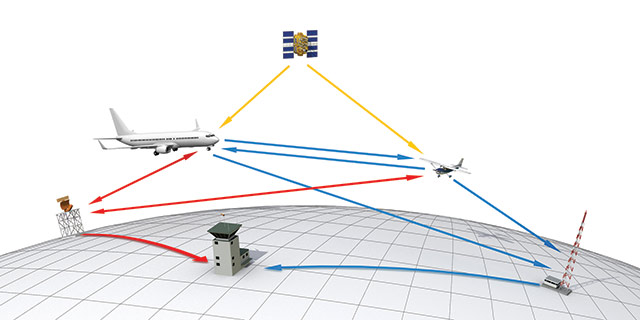
\includegraphics[width=13cm]{pic/Advocacy_ADS_B.jpg}
\caption{ADS-B 系统工作原理}
\label{fig:Advocacy_ADS_B}
\end{figure}

ADS-B 分为两个部分:ADS-B In 和 ADS-B Out。ADS-B In 是系统的接收部分,负责接收 ADS-B 信息;ADS-B Out 是安装有发射器的面板,负责向其他飞机和地面站发送信号,这将告诉其他飞机和地面站本飞行器的位置、速度和航向等信息。注意 ADS-B Out 设备是始终安装在飞机上的并且需要经过认证,这个设备不可拆卸。这样做的目的是为了防止在未授权的情况下,人为关闭 ADS-B 等其他监视跟踪设备,致使无法追踪飞机位置,导致像马来西亚航空 MH370 航班那样的事故。

\subsection{数据链类型}

为了避免频率过载,ADS-B 可以使用不同的数据链以使用不同的频率收/发数据。目前可以支持 ADS-B 技术的数据链主要有三种,分别是基于 S 模式的 1090ES、978UAT(Universal Access Transceiver,通用访问收发机)数据链和 VDL Mode4(VHFDigital Link,模式 4 甚高频数据链)。这三种数据链技术各有优缺点,当前美国同时使用 1090ES 和 UAT 数据链,欧洲同时使用 1090ES 和 VDL Mode4 数据链,而澳大利亚仅使用 1090ES 数据链。目前只有 S 模式 1090ES 数据链获得国际无线电组织的批准,同时国际民航组织对 1090ES 数据链的支持力度最大,标准也最完善。你可以拥有多种 ADS-B 产品:仅 978 In、978 In\&Out、仅 1090ES Out 等等。

\subsubsection{1090ES 数据链}

1090ES 是一个使用扩展震荡信标(Extended Squitter)的改进的 S 模式转发器(使用转发器的 1090MHz 频率),
使用高度要超过 18000 英尺。

\subsubsection{978UAT 数据链}

在美国,18000 英尺以下的高度层使用这种数据链,它在 978MHz 上传输,在技术上称为通用访问收发机(UAT)。

\subsubsection{VDL Mode4 数据链}

模式 4 甚高频数据链是经 ICAO 和 ETSI 标准化的甚高频数据链技术,用于提供移动基站(飞行器和机场地面车辆)、移动单元和固定基站之间的数字通信,它的传输频率在 25 kHz\upcite{h8}。

\section{ADS-B 系统的应用意义}

当前世界范围内空中交通流量与密度不断增加,在未来的几十年内,随着无人机的普及,有人驾驶飞机和无人机都需要在同一片空域正常且无冲突地运行。下一代空中交通管理系统是处理空中流量爆发式增长和保证数十亿乘客安全的关键所在。ADS-B 是这一关键的核心技术,它的出现,将大幅提升航行监视系统的态势感知能力。当前我国民航空中监视系统的中流砥柱是二次雷达,这种基于传统通信模式的的监视设备一般可以报告飞机的身份识别代码、高度代码、飞机地址等信息,由于消息长度限制,不能提供位置完整性报告。为了保持空中交通的效率,同时保证安全,需要提供更精确的监测系统和消息的完整性,ADS-B 可以克服当前雷达系统的局限性并提高其监视性能,增加空域容量,在无法部署雷达的内陆地区,ADS-B 能为飞机提供优于雷达间隔标准的虚拟雷达管制服务;在有雷达覆盖地区,在不增加雷达设备的情况下,能够以较低代价辅助现有雷达系统。ADS-B 系统并非一个独立的监视系统,它对外部系统的高度依赖,比如 GPS 系统将为其提供位置报告,正因为此,ADS-B 的监视精度可以提高至 10 米量级,监视数据更新速度可达 1 秒 1 次。另外,ADS-B 技术成本较低,其地面站建设成本是传统二次雷达的九分之一。ADS-B 技术将为传统空管监视领域带来重大变革。

\section{ADS-B 系统的发展现状}

国际民航组织于第十一届航行大会确定 ADS-B 技术为全球新航行技术的主要发展方向,目前全球各国都在不懈推广 ADS-B 技术的应用。目前对 ADS-B Out 进行强制装备或建议装备的国家越来越多\upcite{h7},部分有 ADS-B Out 装备要求和建议的国家见表\ref{tab:Countries_with_ADS-B_Out_mandates_and_proposals}。

\renewcommand\arraystretch{1.5}
\begin{table}[htbp]
\centering
\caption{部分有 ADS-B Out 装备要求和建议的国家\protect\footnotemark}
\label{tab:Countries_with_ADS-B_Out_mandates_and_proposals}
\begin{tabular}[b]{|p{2cm}<{\raggedleft}|p{13cm}<{\raggedright}|}
\hline
\textbf{美国} & 美国联邦航空局已要求在 2020 年 1 月 1 日之后所有飞机需要装备 ADS-B Out,目前大部分空域需要装备 C 模式转发器。有一个重要的例外情况:在墨西哥湾以上的某个空域也需要 ADS-B。目前,只有美国允许将 978UAT 数据链路用于 ADS-B Out。如果计划在美国以外的 ADS-B 空域飞行,则需要使用 S 模式 1090ES 数据链路 \\
\hline
\textbf{澳大利亚} & 所有 IFR 飞行都需要 1090ES。2020 年 6 月 6 日之前,配备转发器的外国注册飞机在飞行高度低于 FL290 时免于装备 1090ES \\
\hline
\textbf{加拿大} & 目前没有要求,但自愿装备 1090ES(特别是在哈德逊湾和附近的海洋空域)的运营商可以获得更高水平的服务。NAV CANADA 是 Aireon 联合空中交通监控机构的一部分,在低地球轨道卫星上安装 ADS-B 设备。NAV CANADA 将在 2018 年提供服务时成为启动客户,并且最初打算将 1090ES ADS-B 纳入北大西洋空域 \\
\hline
\textbf{欧洲} & MTOW 超过 12566 磅,或最大巡航空速超过 250 节的 IFR 飞机需要装备 1090ES,对于新生产的飞机要求强制装备,并且必须在 2020 年 6 月 7 日之前对所有飞机进行改装 \\
\hline
\textbf{香港} & 所有空域 FL290 及以上需要 1090ES \\
\hline
\textbf{印度尼西亚} & FL290 及以上需要 1090ES \\
\hline
\textbf{墨西哥} & 从 2020 年 1 月 1 日开始,在平均海平面 10000 英尺以上 A、B、C、E 级空域以及其他指定的空域需要 1090ES;目前要求在墨西哥湾的 E 级空域和墨西哥海岸 12 海里以内平均海平面 3000 英尺以上需要 1090ES \\
\hline
\textbf{新加坡} & 指定的航空公司需要 1090ES \\
\hline
\textbf{斯里兰卡} & Colombo 终端控制区(TMA,Colombo Terminal Control Area),FL290 及以上需要需要 1090ES \\
\hline
\textbf{台湾} & 所有空域 FL290 及以上需要 1090ES \\
\hline
\textbf{越南} & 指定的航空公司需要 1090ES \\
\hline
\end{tabular}
\end{table}

\footnotetext{数据来源:\url{https://www.aopa.org/go-fly/aircraft-and-ownership/ads-b/where-is-ads-b-out-required}}

\subsection{国外应用现状}

目前欧美等航空发达国家已制定本国和本地区的 ADS-B 实施规划,建立相关的规章和标准,开展验证与应用。

\subsubsection{北美地区}

在国外,美国是最先开展 ADS-B 技术研究和应用的国家之一,是美国 NextGen 计划的基础之一,帮助飞行员和空中交通管制员创建一个更安全、更高效的国家空域系统(NAS)。美国的 ADS-B 应用路线是:先通用航空,后商用运输。目前,在通用航空方面,美国已经完全实现使用 ADS-B 技术来为自己的航空器提供监视服务。

2016 年 9 月,美国联邦航空局(FAA)开始提供 500 美元奖励,以帮助通用航空运营商支付 ADS-B 设备和安装费用,并鼓励他们现在就装备。

FAA 要求在 2020 年之前,所有在受控空域飞行的飞机都必须安装有 ADS-B OUT,而对 ADS-B In 的安装没有强制要求。

2016 年,FAA 与墨西哥的空中交通服务提供商 SENEAM 合作,使用合资建立的 ADS-B 地面站扩展在墨西哥湾上空的 ADS-B 监视覆盖水平。新的地面站有助于飞行器飞过美国和墨西哥之间的墨西哥湾。

墨西哥的其他地面站对于空中交通路线提供无缝监控覆盖,使海湾地区的容量从每小时 75 架增加到约 85 架。到 2035 年,这些地面站将为美国-墨西哥领空边界提供更多的海湾航班,从而为运营商节省 7000 万美元。增加容量可减少高峰期的延误,从而节省飞机运营成本和乘客时间。

FAA 正在开发 Interval Management,这是一套借助 ADS-B 的能力对航班进行排队和分配的应用软件。间隔管理的精确间距可以在拥挤的空域内实现更高效的飞行路径,并最大限度地提高空域和机场利用率。这些功能需要新的航空电子设备、地面自动化、决策支持系统和程序。FAA 也在探索 ADS-B 在越来越多的商用太空飞行器发射方面的能力。FAA 也在和运营商和其他的 ANSPs 合作,以评估向海洋空域的管制方提供 ADS-B 数据潜在利益。减少分离标准的替代方法包括使用 ADS-B 或使用增强版本 ADS-C。

\subsubsection{澳大利亚}

澳大利亚的 ADS-B 应用水平也达到了很高的程度,该国地广人稀,雷达监视系统建设部署比较薄弱,鉴于这种情况,澳大利亚开始投资部署 ADS-B 系统以配合为数不多的航管雷达设备。

\subsubsection{欧洲}

欧洲各国 ADS-B 应用水平也在大力推进,当前位于欧洲中部的 OpenSky 感知网络的 ADS-B 系统可以捕捉到欧洲大约 30\% 的商业航班,其监视能力相当可观。ADS-B 也是欧洲单一天空计划(SESAR)的基石,欧盟(欧洲共同体和欧控)是 SESAR 的创始人。

欧洲 ADS-B 实施计划要求从 2015 年起,质量大于 5700kg 或速度超过 250 节的新飞行器当在以仪表飞行规则(IFR)下飞行时要装备 ADS-B Out,已经运营的飞机从 2017 年底开始进行改装,在 2020 年 ADS-B 监视系统需要开始运作\upcite{h2}。

\subsection{国内应用现状}

在 ADS-B 技术的研发应用方面,中国民航紧跟国际发展动态,努力与世界接轨。当今 ADS-B 监视技术已在中国民航处于实用阶段,截至 2014 年底,中国民航全行业运输飞机注册架数已达 2370 架,部分已完成 1090ES(1090Mhz Extended Squitter,1090 兆赫扩展断续脉冲)ADS-B OUT 机载设备加改装。中国民航在西部高原地区实施了 B213 航路(成都-拉萨)ADS-B 试验工程和试验运行,并缩小了航路间隔;在 B330 成都-九寨航路、南中国海开展了 ADS-B 试验验证工作。2015 年,中国民用航空 ADS-B 实施规划颁布,是指导中国民航 ADS-B 实施的纲领性文件。

\subsection{技术发展现状}

在硬件设备的发展上,由于 ADS-B 非独立监视的特性,就像接收广播一样,只要找到合适的设备,用户就可以通过各种渠道接收 ADS-B 信号,由于其技术门槛与
成本相对较低,所以 ADS-B 技术目前被广泛推广。在硬件方面,虽然商用 ADS-B 接收器比较昂贵,但是相较于雷达这种高度精密的设备,其成本也大大降低了。事实上,目前通过一些廉价的接收设备,比如数字电视棒,也可以接收 ADS-B 信号。国内外许多厂家也推出了廉价的 ADS-B 接收设备,例如 RTL-SDR、AirNav RadarBox、三航雷达等。目前国内在民航局政策与标准引导下,工业界已基本具备 ADS-B 设备产业化能力。

\section{全球 ADS-B 覆盖情况}

本小节将介绍世界上几个典型的国家和地区的 ADS-B 实施情况。

\subsection{全球}

全球 ADS-B 覆盖情况如图\ref{fig:1ADS-B-coverage}所示。

\begin{figure}[htbp]
\centering
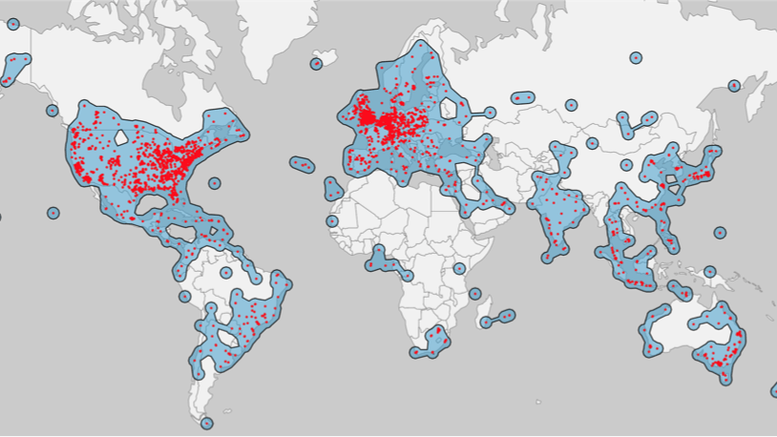
\includegraphics[width=14cm]{pic/1ADS-B-coverage.png}
\caption{全球陆基 ADS-B 覆盖情况\protect\footnotemark}
\label{fig:1ADS-B-coverage}
\end{figure}

\footnotetext{图片来源:\url{https://jdasolutions.aero/blog/ads-b-update-bits-information-around-world/}}

\subsection{澳大利亚}

ADS-B 地面站是视距(line-of-sight)\footnote{通常指波的传播路径为直线,不能沿曲线或者跨障碍物行进}设施,地面站接收下行 ADS-B 数据的能力取决于飞机的高度、飞机与地面站的距离以及障碍物。在海拔较低的低空区域(接近地面),覆盖范围在距离地面站 20 海里半径内,高空空域覆盖半径可以超过 250 海里。

在雷达覆盖范围与 ADS-B 覆盖范围重叠的空域,雷达探测到的飞机位置将会提交给 ATC。

截至 2017 年 1 月,澳大利亚纯 ADS-B 覆盖区域如图\ref{fig:ADS-B-5000}、\ref{fig:ADS-B-10k}、\ref{fig:ADS-B-20k}、\ref{fig:ADS-B-30k}所示,澳大利亚 30000 英尺以上高空已实现 ADS-B 密集覆盖,航路管制间隔已缩至 5 海里水平。

\begin{figure}[htbp]
\centering
\begin{minipage}[t]{0.48\textwidth}
\centering
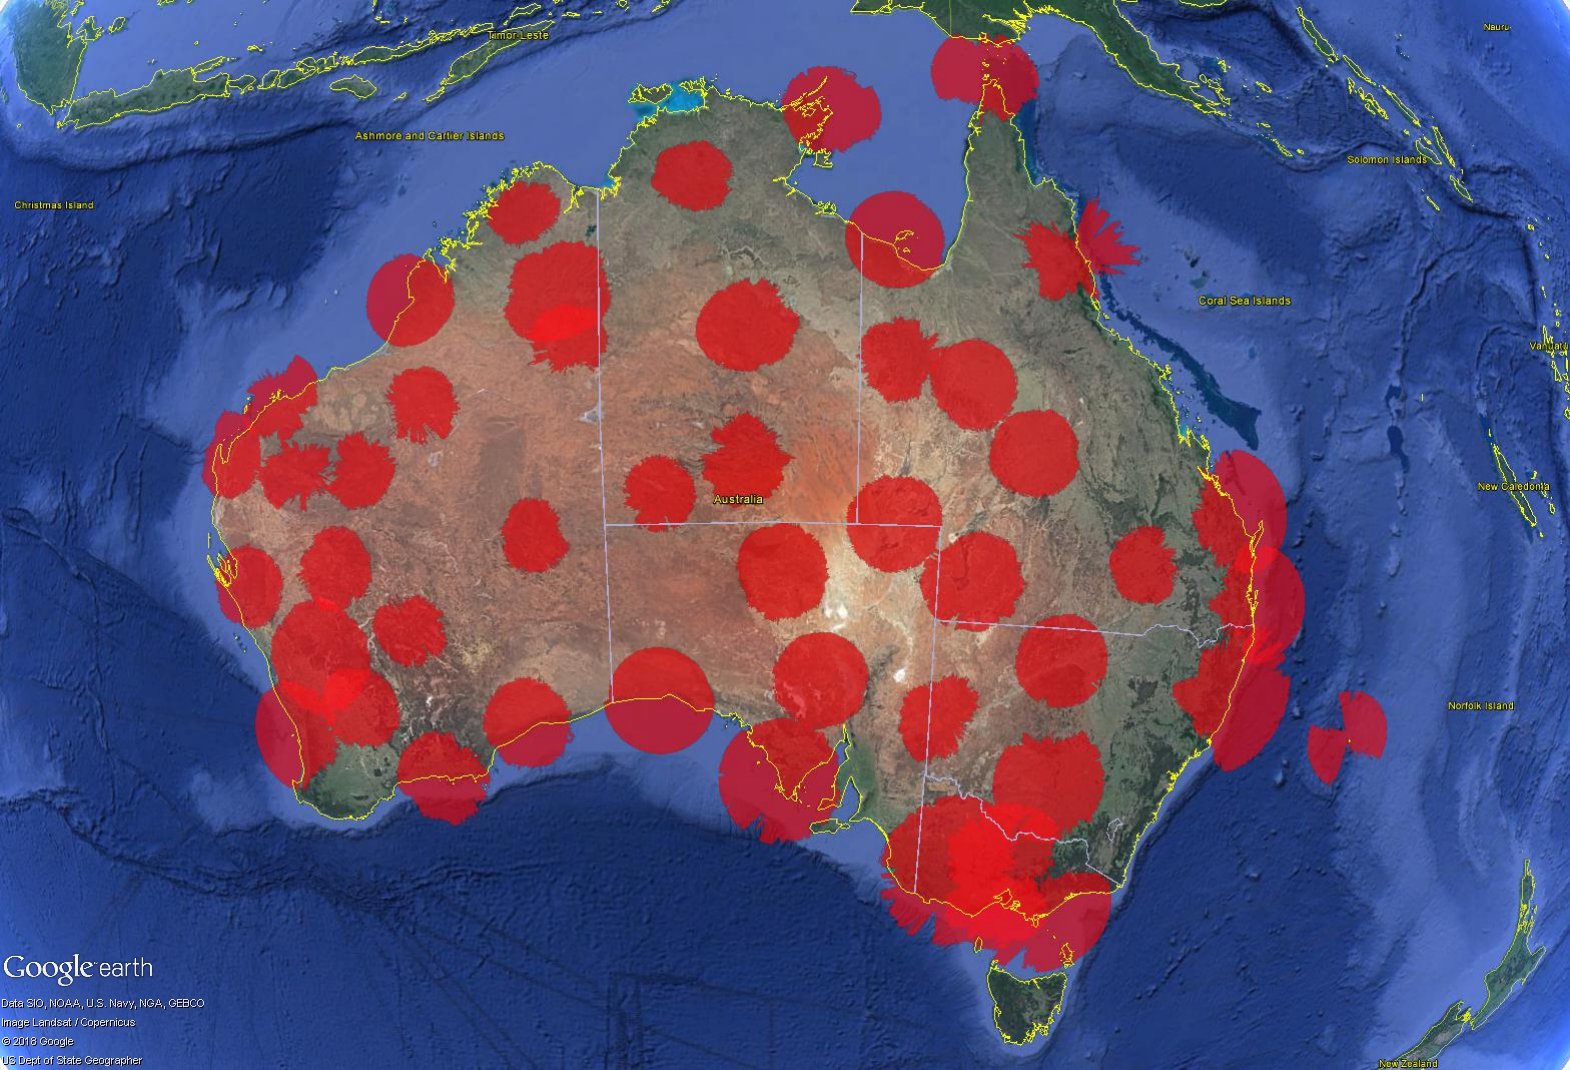
\includegraphics[width=7.5cm]{pic/ADS-B-5000.jpg}
\caption{澳洲 5000ft 空域覆盖范围\protect\footnotemark}
\label{fig:ADS-B-5000}
\end{minipage}
\begin{minipage}[t]{0.48\textwidth}
\centering
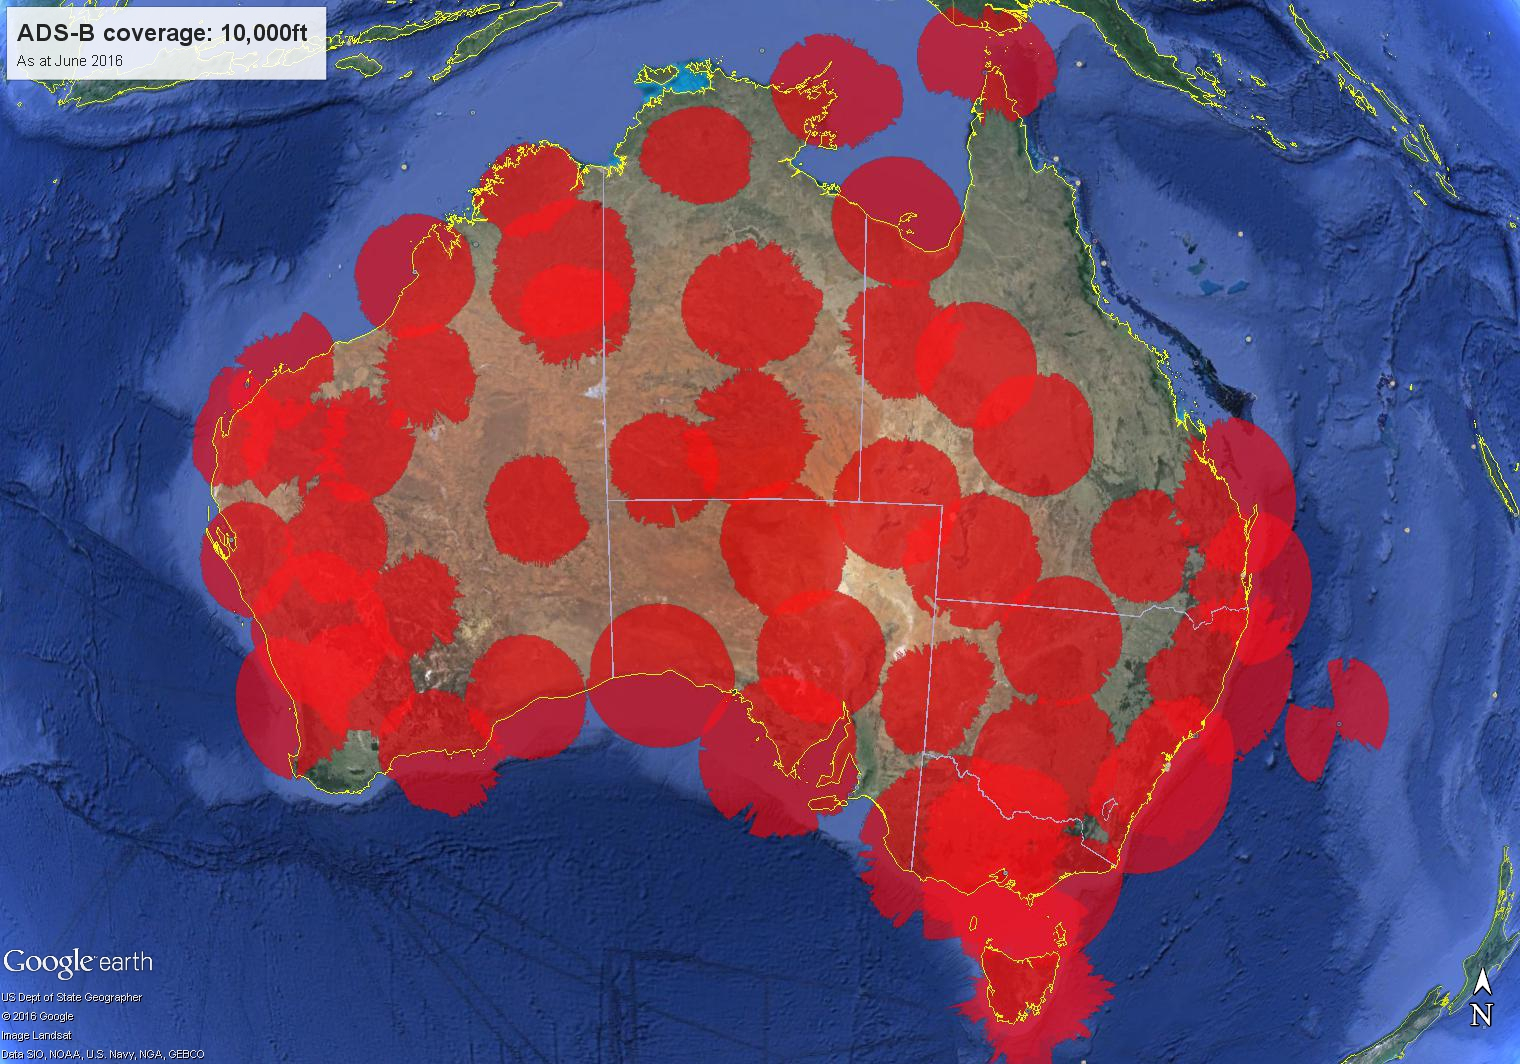
\includegraphics[width=7.5cm]{pic/ADS-B-10k.jpg}
\caption{澳洲 10000ft 空域覆盖范围}
\label{fig:ADS-B-10k}
\end{minipage}
\end{figure}

\begin{figure}[htbp]
\centering
\begin{minipage}[t]{0.48\textwidth}
\centering
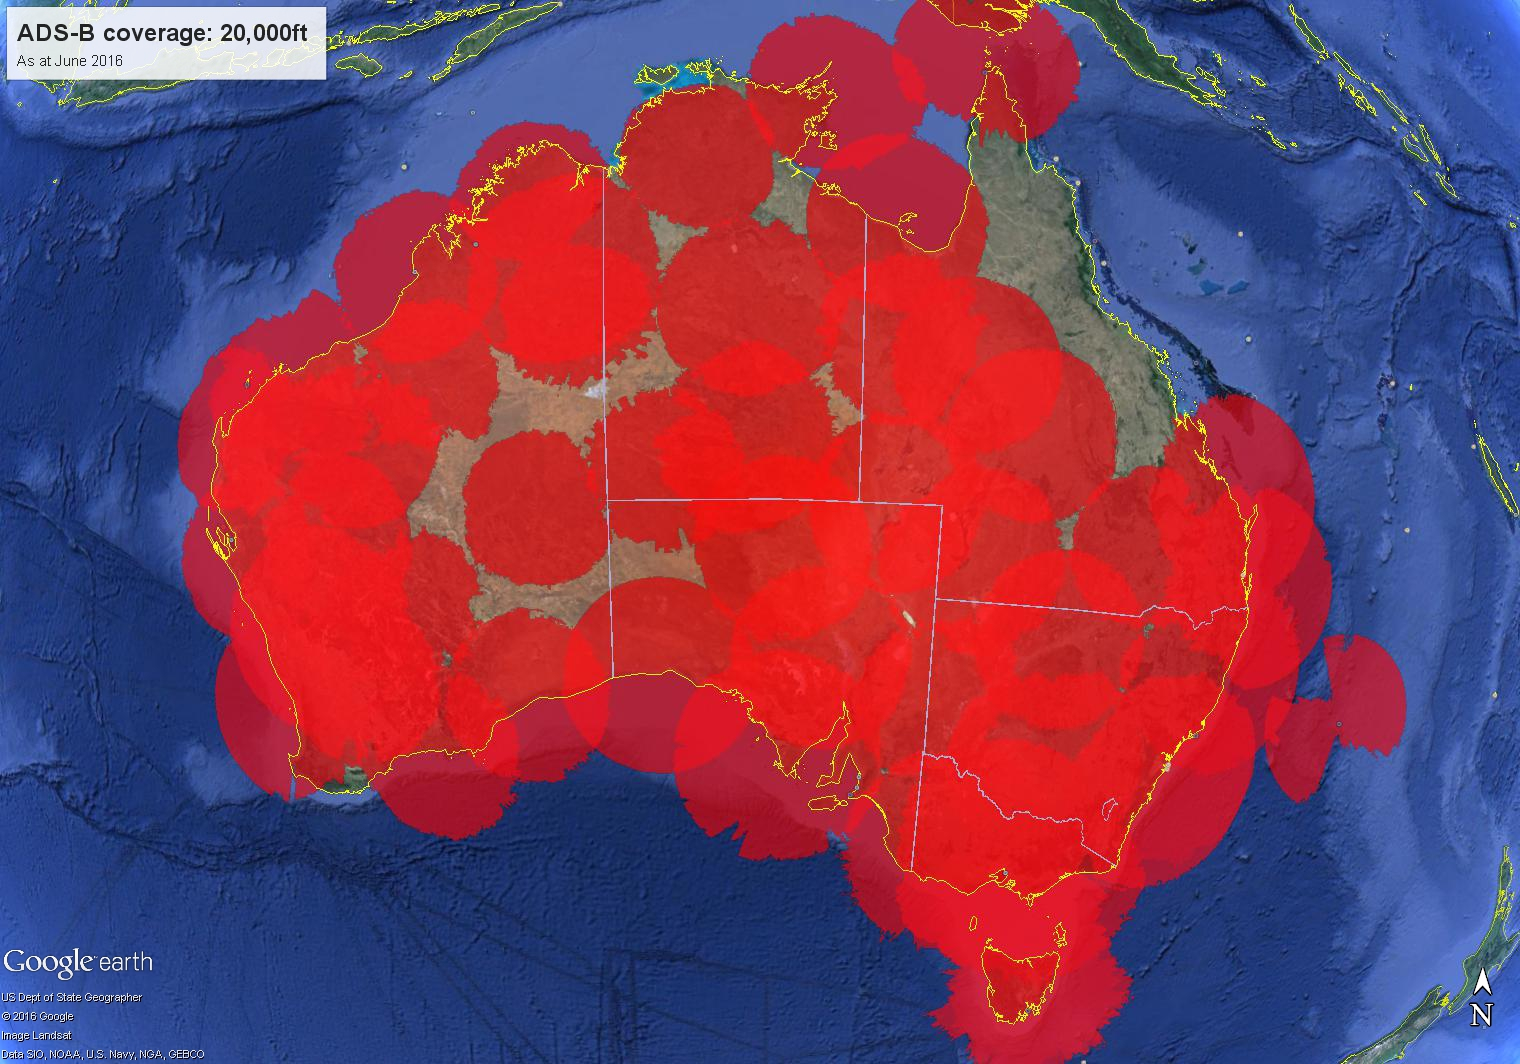
\includegraphics[width=7.5cm]{pic/ADS-B-20k.jpg}
\caption{澳洲 20000ft 空域覆盖范围}
\label{fig:ADS-B-20k}
\end{minipage}
\begin{minipage}[t]{0.48\textwidth}
\centering
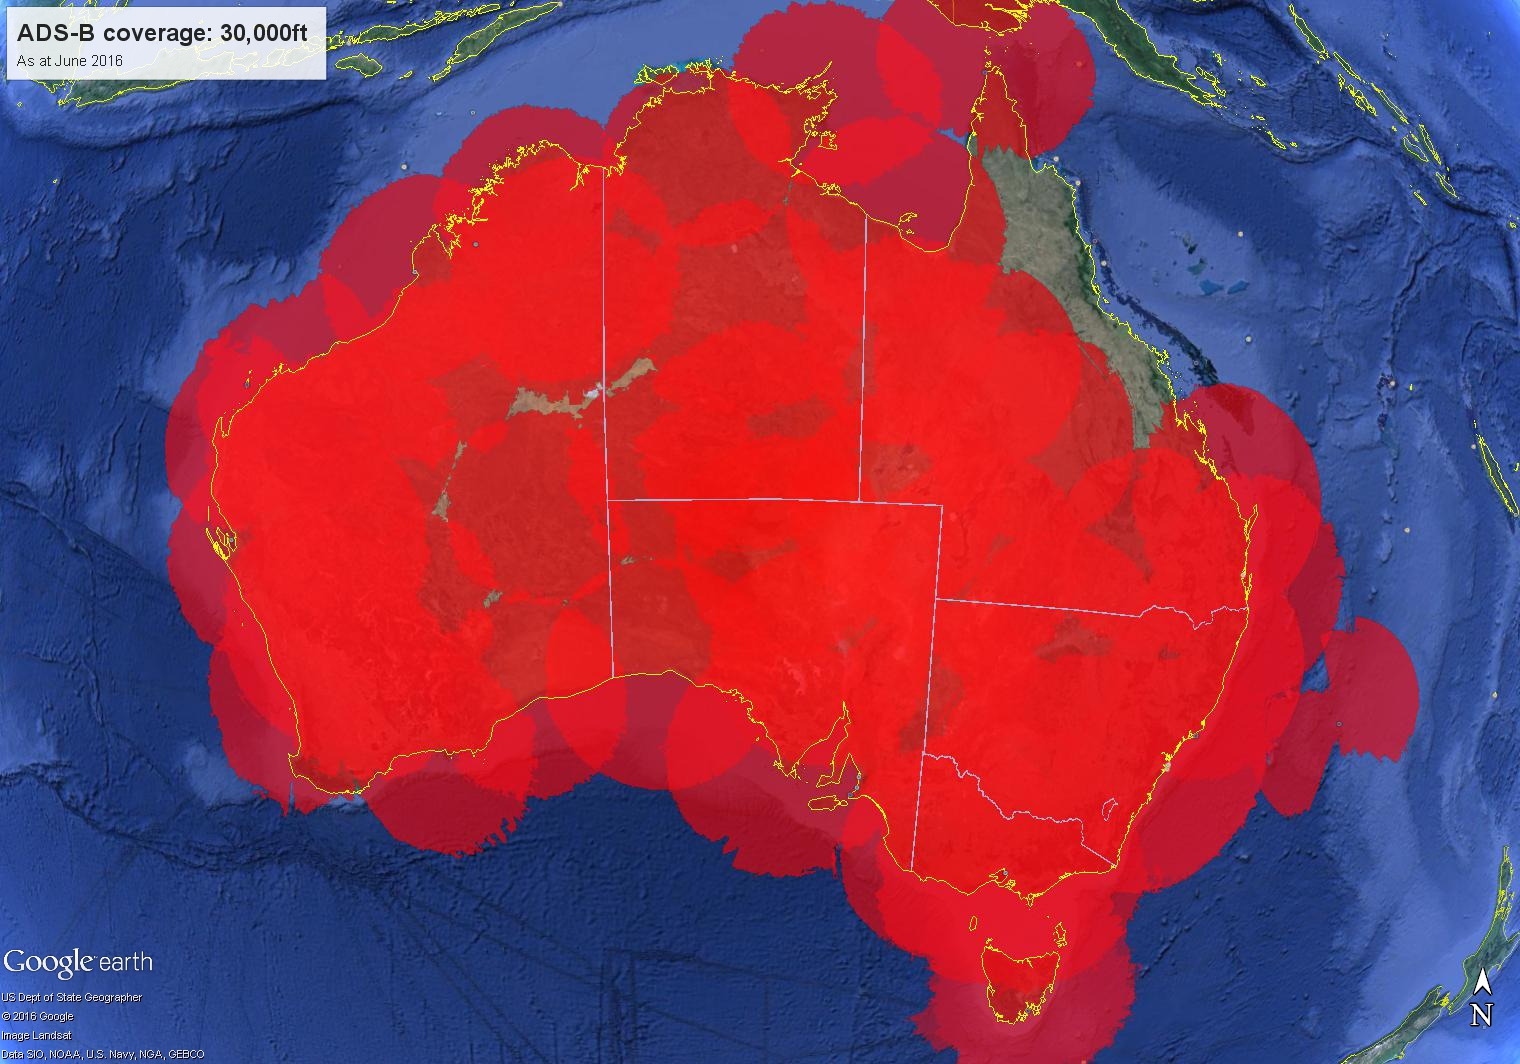
\includegraphics[width=7.5cm]{pic/ADS-B-30k.jpg}
\caption{澳洲 30000ft 空域覆盖范围}
\label{fig:ADS-B-30k}
\end{minipage}
\end{figure}

\footnotetext{图片来源:\url{http://www.airservicesaustralia.com/projects/ads-b/ads-b-coverage/}}

\subsection{北美地区}

截至 2017 年 4 月,ADS-B 在美国全境的覆盖情况如图\ref{fig:ADS-B-Coverage-Area}所示。

\begin{figure}[htbp]
\centering
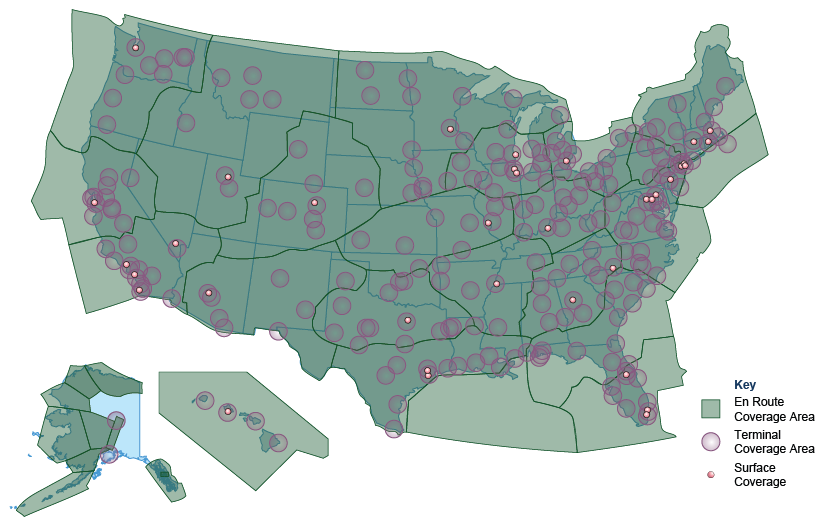
\includegraphics[width=14cm]{pic/ADS-B-Coverage-Area.png}
\caption{美国陆基 ADS-B 覆盖情况\protect\footnotemark}
\label{fig:ADS-B-Coverage-Area}
\end{figure}

\footnotetext{图片来源:Corporate Fleet Service(CFS),\url{http://cfsjets.com/2017/12/14/ads-b-where-we-are-now//}}

根据美国麻省理工学院 2011 年 6月的一份报告\upcite{e3}显示,预计 ADS-B 在美国全面实施后其覆盖情况如图\ref{fig:ADSB-final}所示。

\begin{figure}[htbp]
\centering
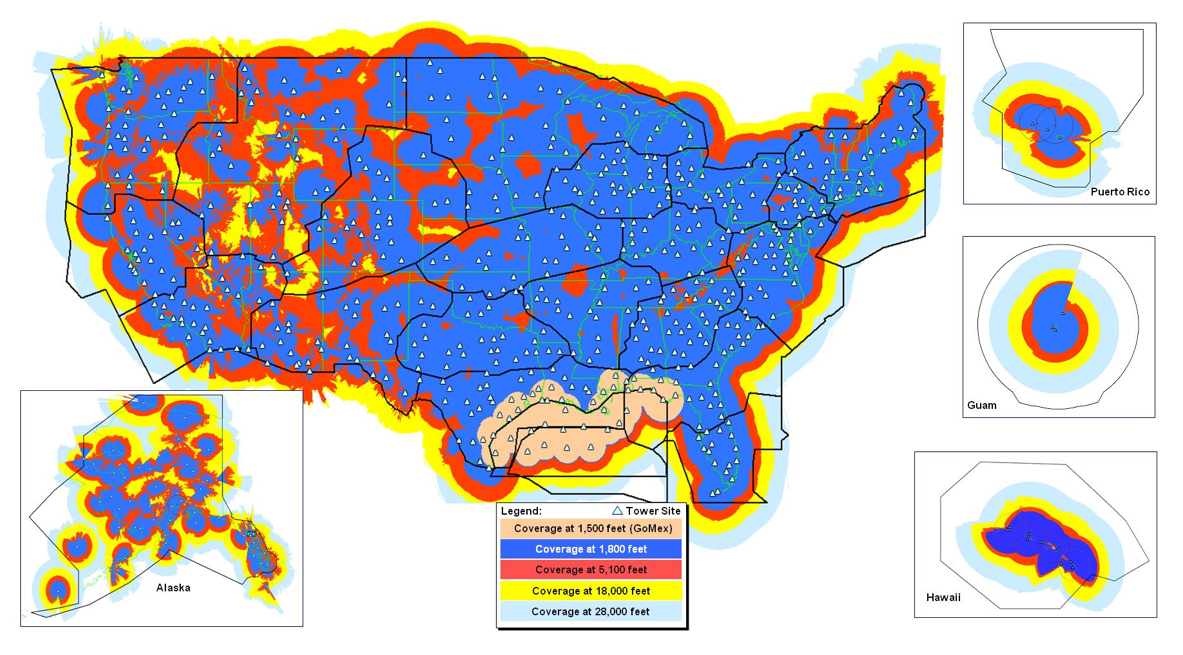
\includegraphics[width=14cm]{pic/ADSB-final.png}
\caption{预测的 ADS-B 全面实施后的覆盖率\protect\footnotemark}
\label{fig:ADSB-final}
\end{figure}

\footnotetext{图片来源:参考文献\cite{e3,e4}}

更为详细的 ADS-B 覆盖情况可以在 FAA 网站\footnote{\url{https://www.faa.gov/nextgen/programs/adsb/}}上查询,它提供了一个动态的可交互式的 ADS-B 覆盖范围查询网页。

\subsection{欧洲}

\subsubsection{现阶段}

\begin{itemize}

    \item \textbf{地面段 ADS-B(基站部署)- 空域和机场监视}

    2018 年 5 月 15 日的 SESAR 关于欧洲 ADS-B 系统建设的阶段性报告展示了欧洲 ADS-B 系统的相关情况\upcite{e5}。

    图\ref{fig:20180515-sesar-ads-b-report_18}显示了欧洲 ADS-B 监控系统的实施现状、相关覆盖范围,以及 ATM 系统中相关监控数据的集成水平。

    \begin{figure}[htbp]
    \centering
    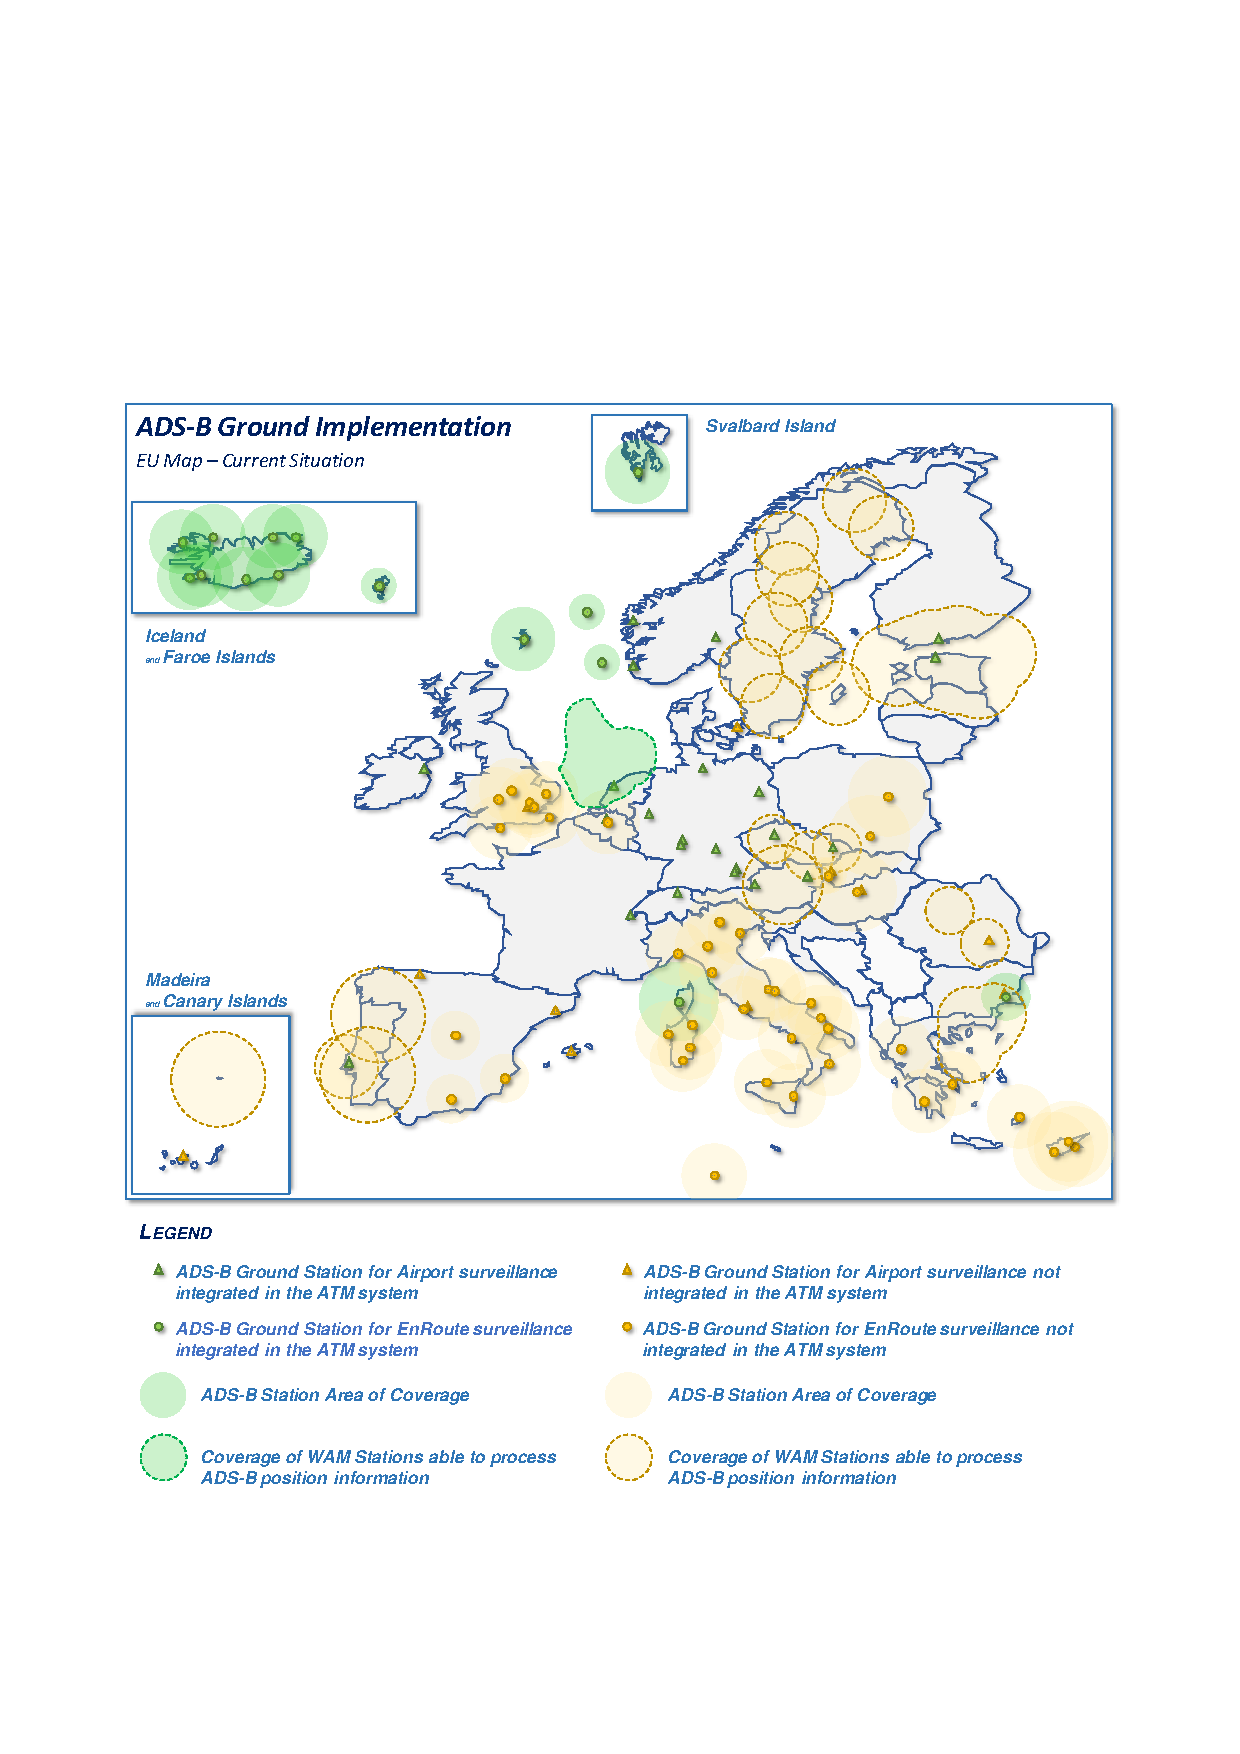
\includegraphics[width=14cm]{pic/20180515-sesar-ads-b-report_18.pdf}
    \caption{欧洲 ADS-B 地面监控系统的实施现状\protect\footnotemark}
    \label{fig:20180515-sesar-ads-b-report_18}
    \end{figure}

    \footnotetext{图片来源:参考文献\cite{e5}}

    \begin{itemize}
        \item \textbf{空域 ADS-B 监视}

        欧洲 ADS-B 接收机的安装现状比较零散。总共安装了 70 多个具备航路 ADS-B 监控能力的基站,其中约 90\% 在运行中,其余 10\% 用于测试和验证。现有 ADS-B 站的剩余平均寿命为 12 年。

        \item \textbf{机场 ADS-B 监视}

        用于机场监控的 ADS-B 系统非常广泛,目前,欧洲共安装了 34 个机场 ADS-B 站:其中 23 个被集成到 ATM 系统中,11 个没有被集成到 ATM 系统中,但计划将它们与 MLAT 系统集成。机场 ADS-B 在与 ATM 系统集成时,无论是否与 MLAT 结合,都只用于地面车辆的识别和定位数据,因为数据质量要求没有飞机那么严格。现有 ADS-B 站的剩余平均寿命为 8 年。
    \end{itemize}

    \item \textbf{空中段 ADS-B(机上终端)}

    图\ref{fig:airborne-ads-b-euro}显示了符合 ADS-B ED-102A(DO-260B)规定的 ADS-B 应答器的实施现状,该应答器共装备于 35 家总部位于欧盟的航空公司的共 3108 架飞机上。

    \begin{figure}[htbp]
    \centering
    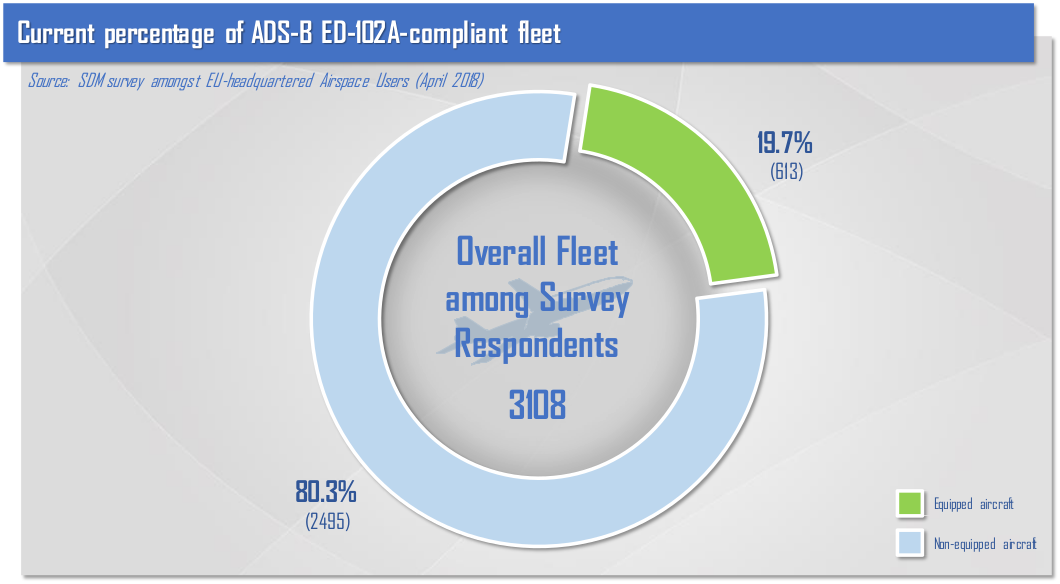
\includegraphics[width=16cm]{pic/airborne-ads-b-euro.png}
    \caption{欧洲各国现阶段飞机 ADS-B 终端装备情况\protect\footnotemark}
    \label{fig:airborne-ads-b-euro}
    \end{figure}

    \footnotetext{图片来源:参考文献\cite{e5}}

    \item \textbf{星基 ADS-B}

    关于星基 ADS-B 信息的地面使用情况,28 家 ANSP 在回答问卷时表示,15 家 ANSP 没有使用星基 ADS-B 数据的计划,而 13 家 ANSP 表示,一旦服务可用,他们正在考虑使用该数据。

    NATS 和 NAV CANADA 计划在 2019-2020 年期间在北大西洋和加拿大部署星基 ADS-B (Aireon)。一些欧洲的 ANSP 计划从 2019 年第一季度开始使用它。

\end{itemize}

\subsubsection{2020 年及以后}

\begin{itemize}

    \item \textbf{2020 年地面段 ADS-B(基站部署)- 空域和机场监视}

    图\ref{fig:20180515-sesar-ads-b-report_33}显示了利益攸关方在全欧洲实施 ADS-B 监控系统的短期计划。特别是,该图包括所有预计在 2020 年之前安装和/或运行的 ADS-B 系统。

    \begin{figure}[htbp]
    \centering
    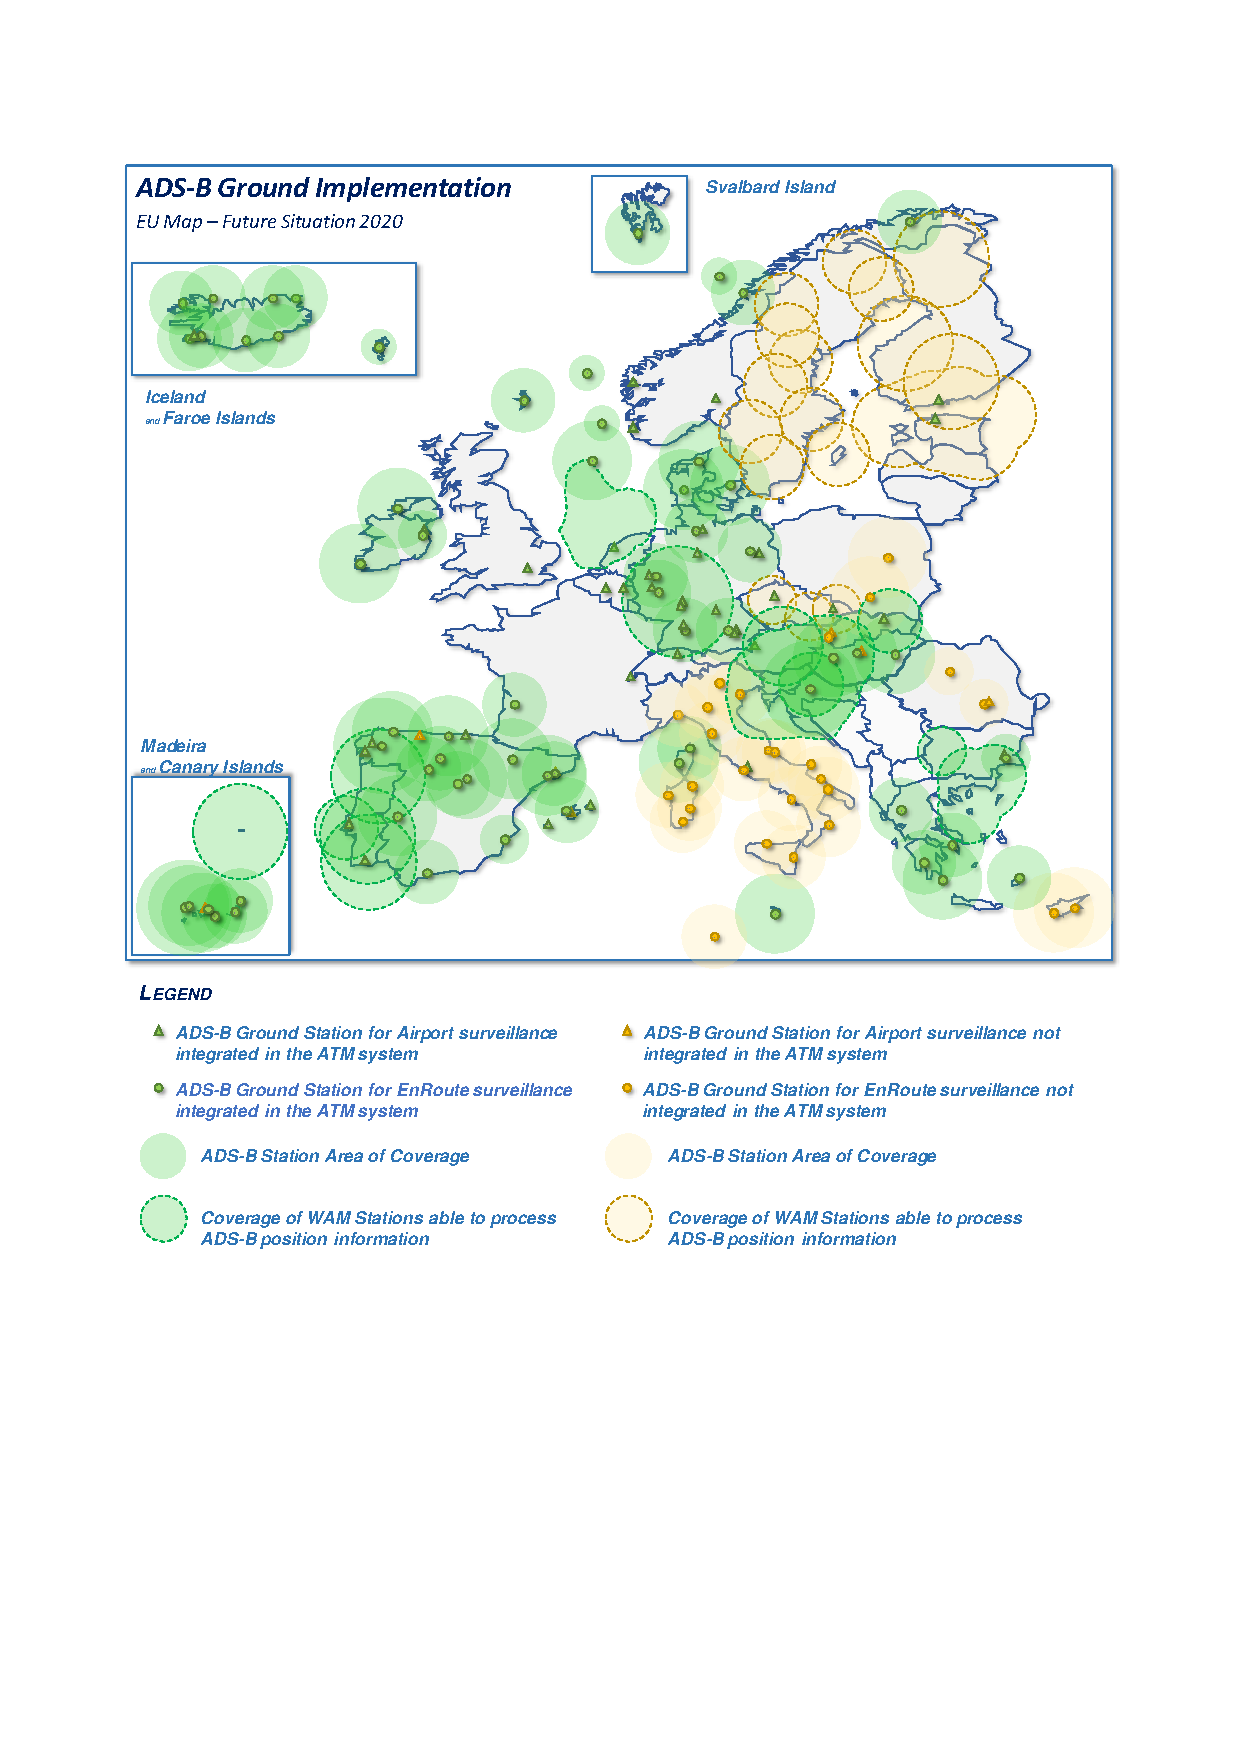
\includegraphics[width=15cm]{pic/20180515-sesar-ads-b-report_33.pdf}
    \caption{欧洲 2020 年 ADS-B 地面监控系统实施计划\protect\footnotemark}
    \label{fig:20180515-sesar-ads-b-report_33}
    \end{figure}

    \footnotetext{图片来源:参考文献\cite{e5}}

    \begin{itemize}
        \item \textbf{空域 ADS-B 监视}

        未来欧洲 ADS-B 接收机的安装情况显示,采用 ADS-B 的趋势越来越明显。在 ANSP 的投资计划中,总共有 60 多个具备 ADS-B 能力的航路监测站。值得强调的是,由 WAM 或 ADS-B 基站顶部的 S 模式雷达将提供大量计划中的 ADS-B 功能。

        ADS-B 基站的典型寿命为 15-18 年。

        \item \textbf{机场 ADS-B 监视}

        作为上述投资的补充,ANSP 和机场运营商计划在 2018 年至 2020 年间安装/更新大约 25 个 ADS-B 站,用于机场监控。这些监测站将补充和/或取代现有的基础设施,并将扩大 ADS-B 在欧洲机场的覆盖范围。

        在短期内,ADS-B 基础设施将继续集成到 ATM 系统中,首先跟踪车辆的位置,然后将其增强到飞机上。从 2018 年起,现有 ADS-B 站的剩余平均寿命为 15 年。
    \end{itemize}

    \item \textbf{2020 年以后地面段 ADS-B(基站部署)- 空域和机场监视}

    图\ref{fig:20180515-sesar-ads-b-report_35}补充了前一段展示的短期规划,包括业务利益相关者在未来数年实施 ADS-B 监测系统的长期计划。特别地,该图包括了所有 ADS-B 系统,预计从 2021 年开始安装和运行。

    \begin{figure}[htbp]
    \centering
    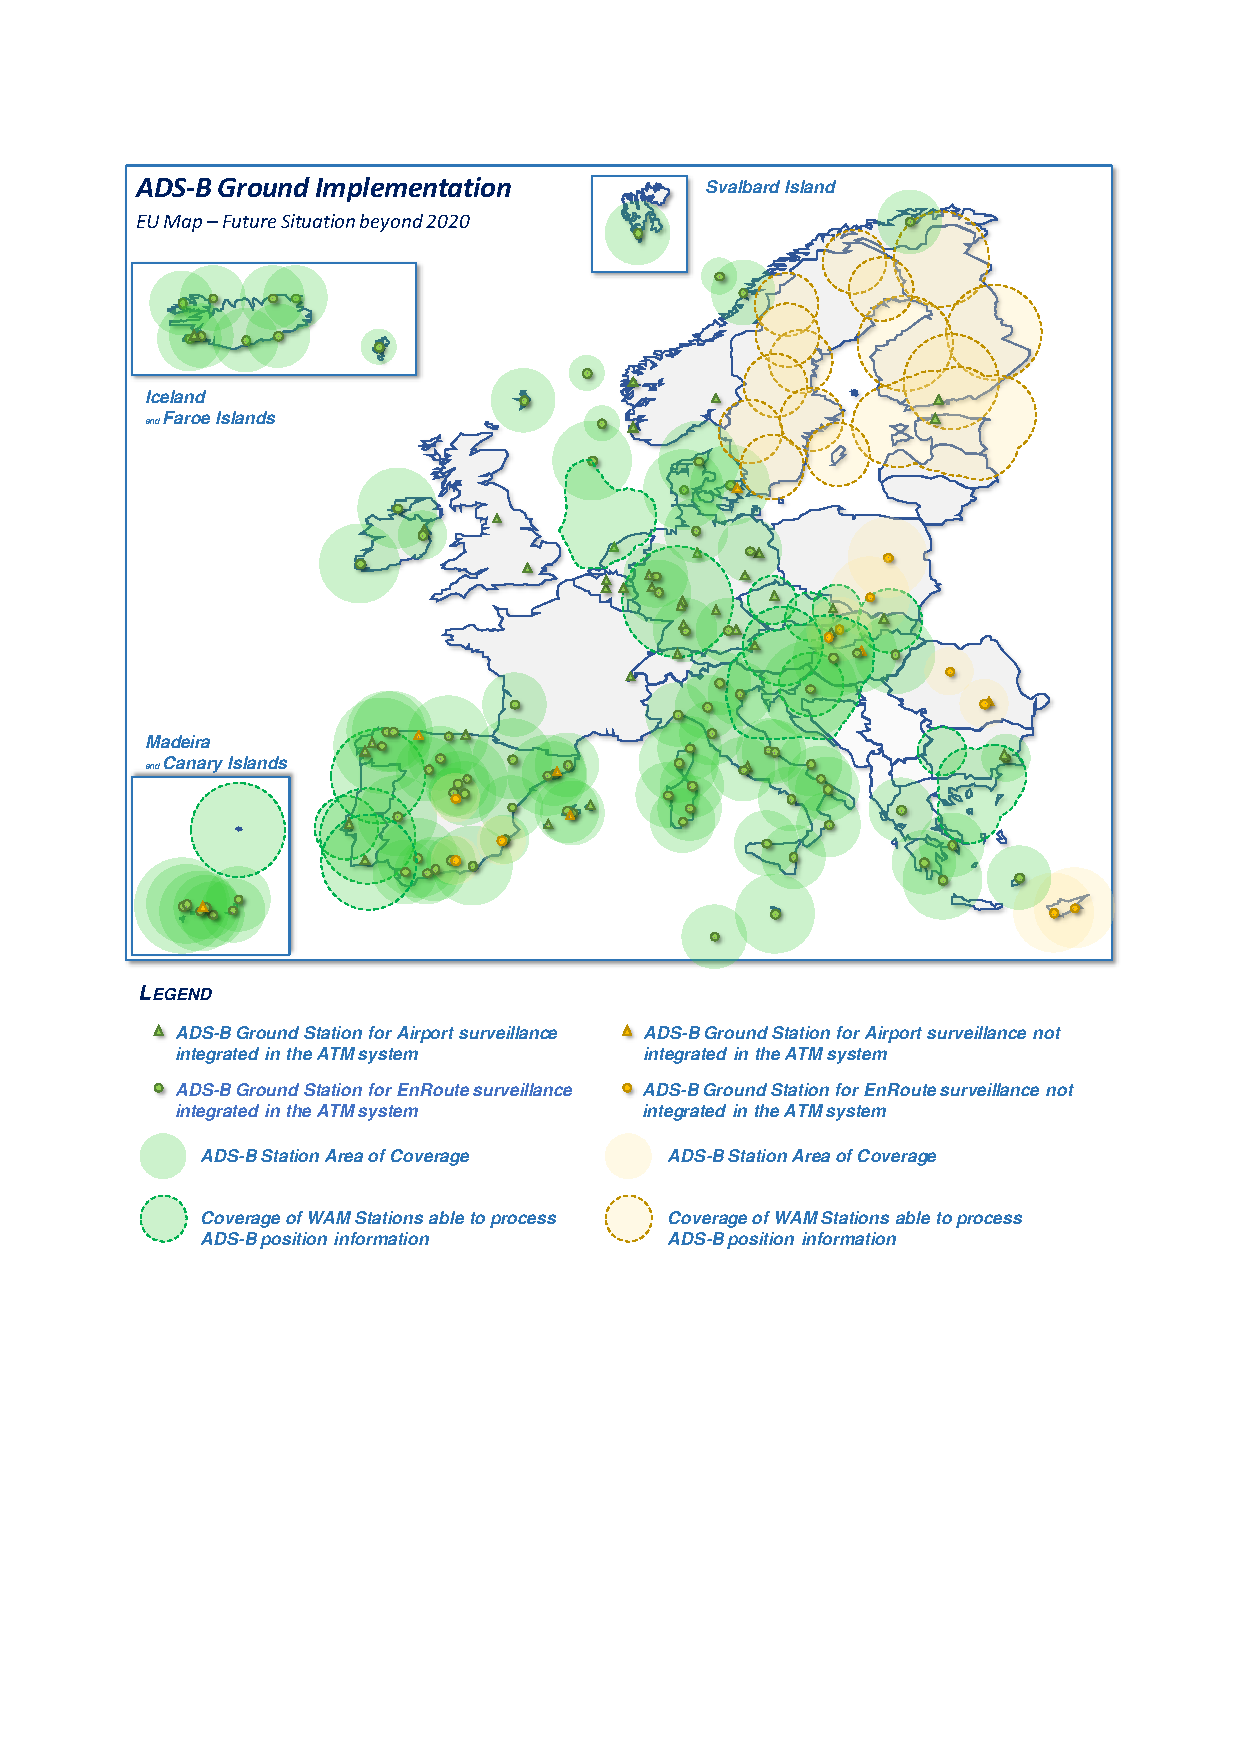
\includegraphics[width=15cm]{pic/20180515-sesar-ads-b-report_35.pdf}
    \caption{欧洲 2020 年之后 ADS-B 地面监控系统实施计划\protect\footnotemark}
    \label{fig:20180515-sesar-ads-b-report_35}
    \end{figure}

    \footnotetext{图片来源:参考文献\cite{e5}}

    \begin{itemize}
        \item \textbf{空域 ADS-B 监视}

        与 2020 年的情况相比,欧洲的 ADS-B 前景略有改善,计划在航线上安装几个具有 ADS-B 能力的监测站。

        西班牙计划增加新的 ADS-B 站,覆盖南部空域(通过在新安装的 S 模式雷达内集成 ADS-B 接收器)。另一方面,意大利和捷克共和国将在业务上使用 ADS-B 数据,从而将信息集成到 ATM 系统中。最后,一个能够接收 ADS-B 数据的额外 WAM 站将覆盖芬兰东部领空,但是没有将这些信息纳入 ATM 系统。

        \item \textbf{机场 ADS-B 监视}

        为配合上述情况,机场服务供应商及机场运营商计划于 2021 年至 2030 年期间安装/更新 6 个 ADS-B 监测站,进行机场监察。这些监测站将补充和/或取代现有的基础设施,并将扩大 ADS-B 在欧洲的覆盖范围。从2018年起,现有ADS-B站的剩余平均寿命为16年。
    \end{itemize}

    \item \textbf{空中段 ADS-B(机上终端)}

    在未来,各主要航空公司正计划顺应规定对新飞机安装 ADS-B,而对现有飞机进行“翻新计划”的情况则有所不同。欧盟可能决定将 2020 年至 2025 年的过渡期延长 5 年,并进一步豁免 2025 年之前退役的飞机,由此引发的预期进一步放大了这一设想,导致该法规再次修订。

    除欧盟和美国外,ADS-B Out(DO-260B应答器)在中国、澳大利亚或日本等其他国家也有或将被授权使用。

    \item \textbf{星基 ADS-B}

    一些 ANSP 正在考虑基于 ADS-B 的空间服务,并且正在进行调查(基于 Aireon 的服务可用性)。三家 ANSP 正计划使用基于空间的 ADS-B。在意大利,星基 ADS-B 系统将集成在 ATS 测试平台上,预计 2020 年后的业务用途将作为地面独立的 ATS 监视层,用于应急和增强监视。中期而言,这可能是传统监控基础设施全球优化的一部分。

\end{itemize}

\subsection{中国}

根据 ICAO 第十五次 ADS-B 研究和实施研讨会议信息论文(IP,Information Paper)显示\upcite{e6},CAAC 于 2015 年 12 月修订了《中国民用航空 ADS-B 实施方案》。根据国家 ADS-B 建设项目审批及实施进度,主要修改是调整各阶段的实现时间。

\begin{itemize}
    \item \textbf{第一阶段}:2017 年底,ADS-B 在中国开始初步运营,以及在 ATS 路线上实施 ADS-B :B213、B345、B215、A460、H66、L888、H15、Z1、B206、A368、M771、L642、N892 和 A1。

    \item \textbf{第二阶段}:2017 年至 2020 年,重点任务是全面推进 ADS-B Out,并对 ADS-B Out 进行安全评估。

    \item \textbf{第三阶段}:2020 年至 2025 年,建成完善的 ADS-B 运营监控系统和信息服务系统,为航空公司提供全空域监控手段和综合 ADS-B 信息服务,增强空中交通管制安全保障能力和服务水平。
\end{itemize}

2017 年底(阶段一)将部署 310 个 ADS-B 地面站、2 个 ADS-B 主数据处理中心、8 个 ADS-B 次数据处理中心。本阶段全国 ADS-B 覆盖率如图\ref{fig:china_3300m}、\ref{fig:china_6600m}、\ref{fig:china_8400m}所示。

\begin{figure}[htbp]
\centering
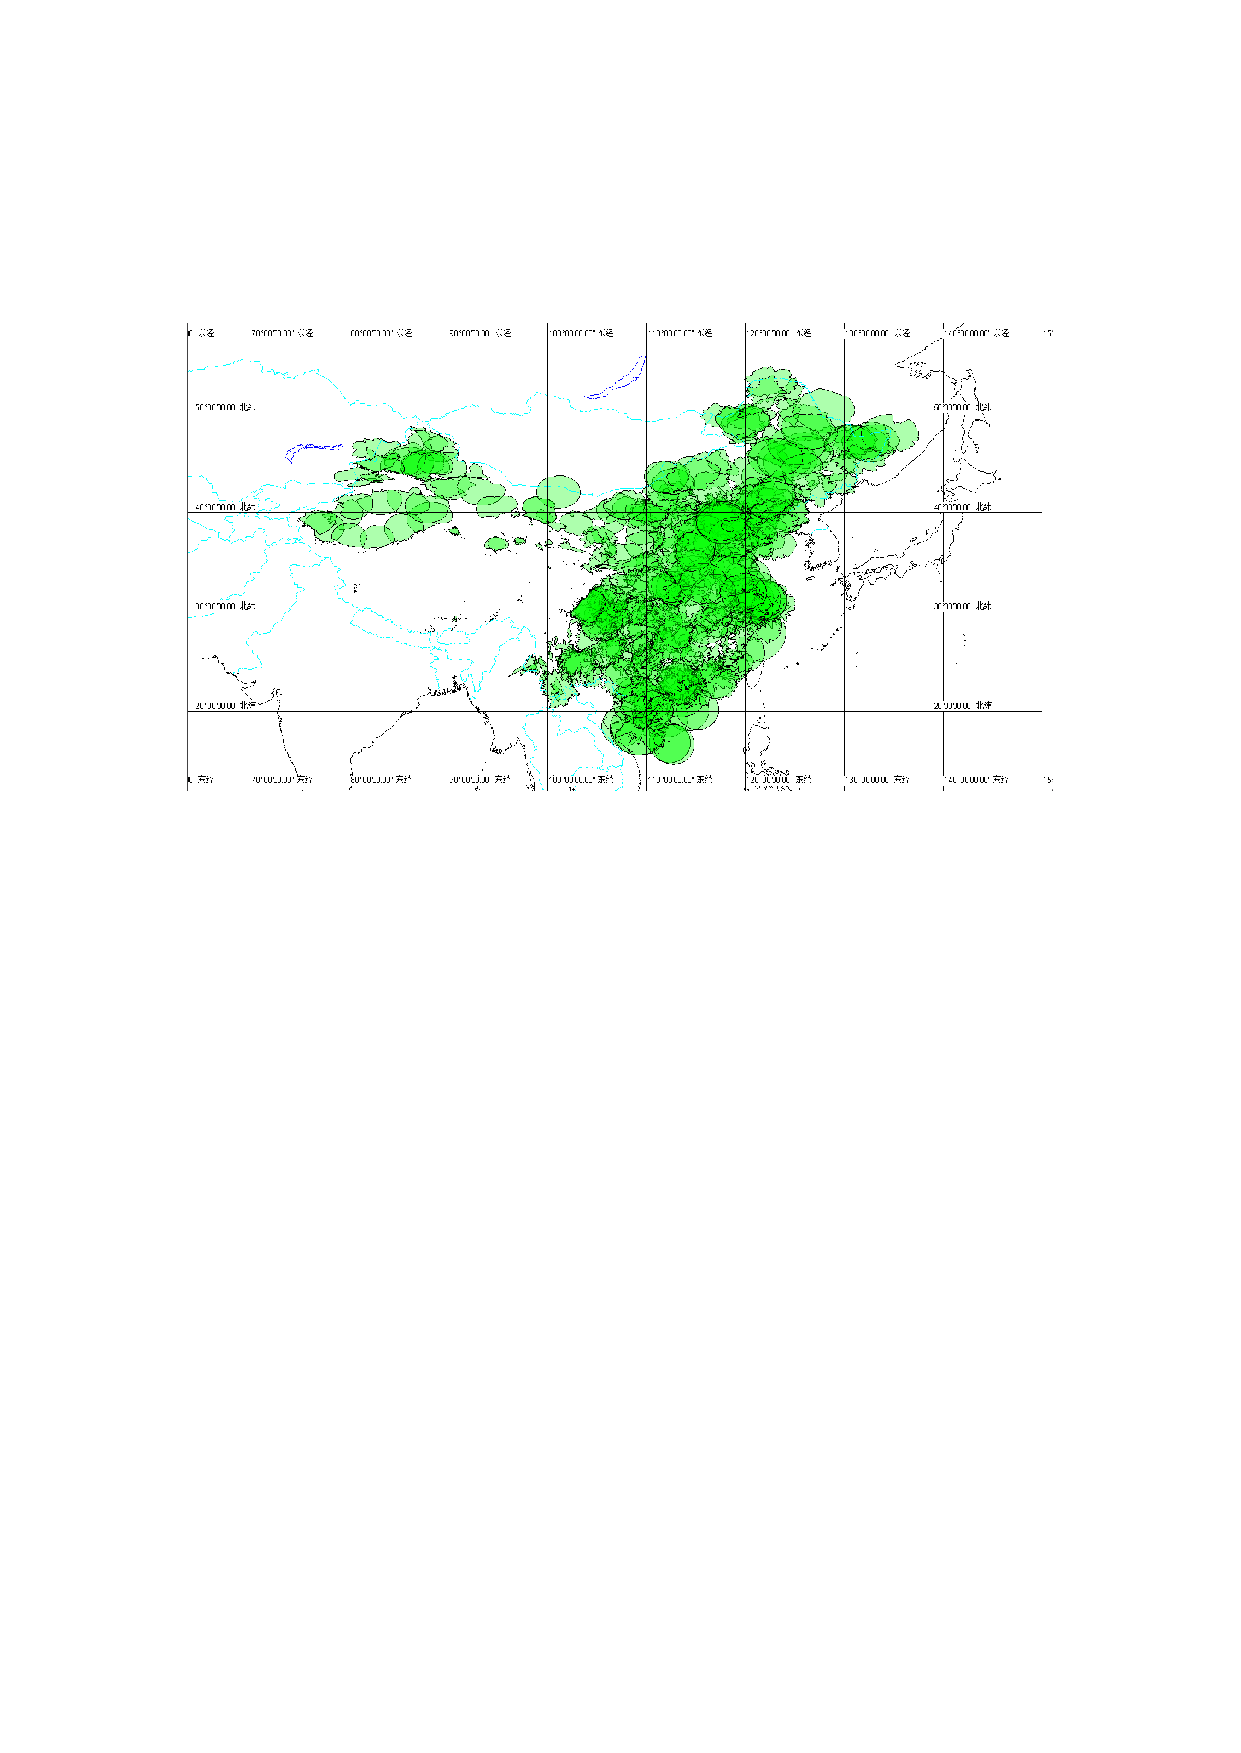
\includegraphics[width=12cm]{pic/china_3300m.pdf}
\caption{中国 3300m 空域 ADS-B 覆盖情况\protect\footnotemark}
\label{fig:china_3300m}
\end{figure}

\footnotetext{图片来源:参考文献\cite{e6}}

\begin{figure}[htbp]
\centering
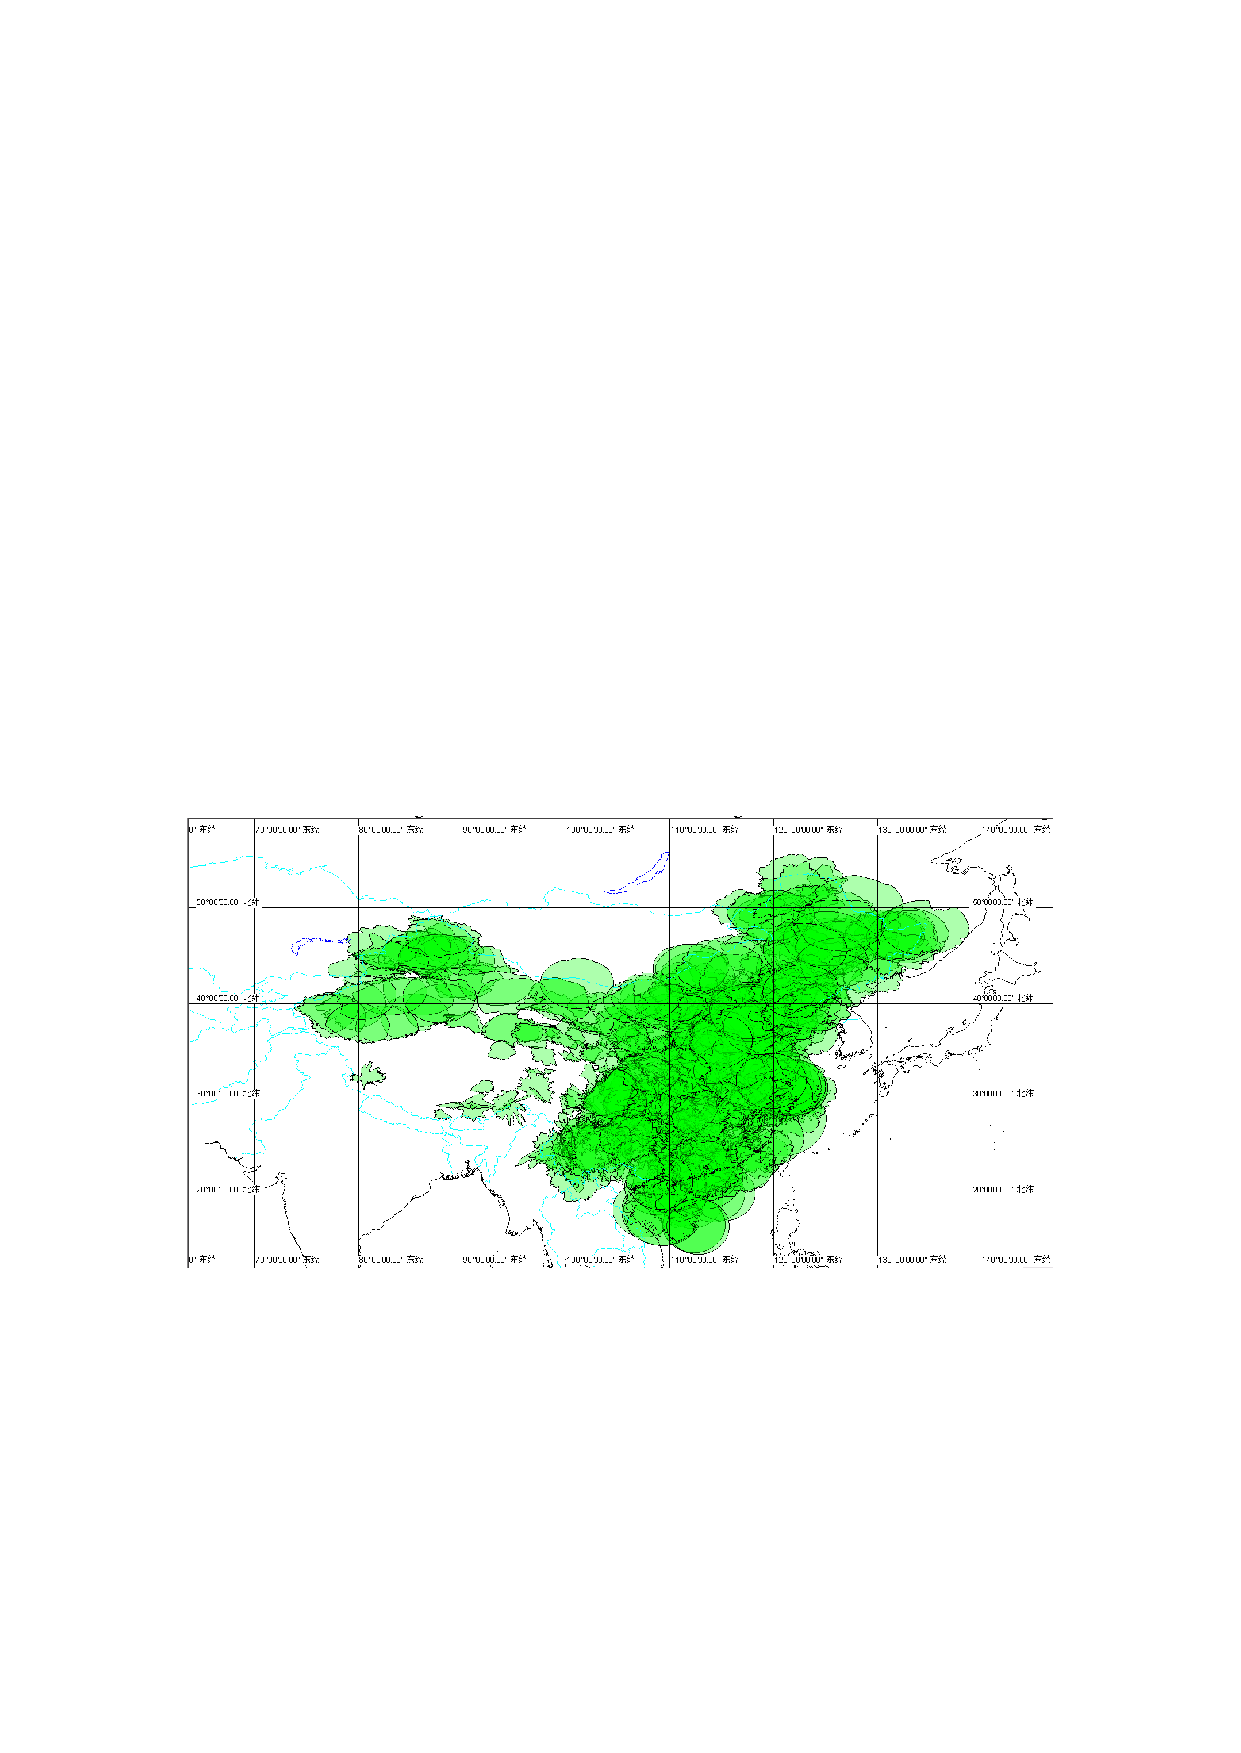
\includegraphics[width=12cm]{pic/china_6600m.pdf}
\caption{中国 6600m 空域 ADS-B 覆盖情况\protect\footnotemark}
\label{fig:china_6600m}
\end{figure}

\footnotetext{图片来源:参考文献\cite{e6}}

\begin{figure}[htbp]
\centering
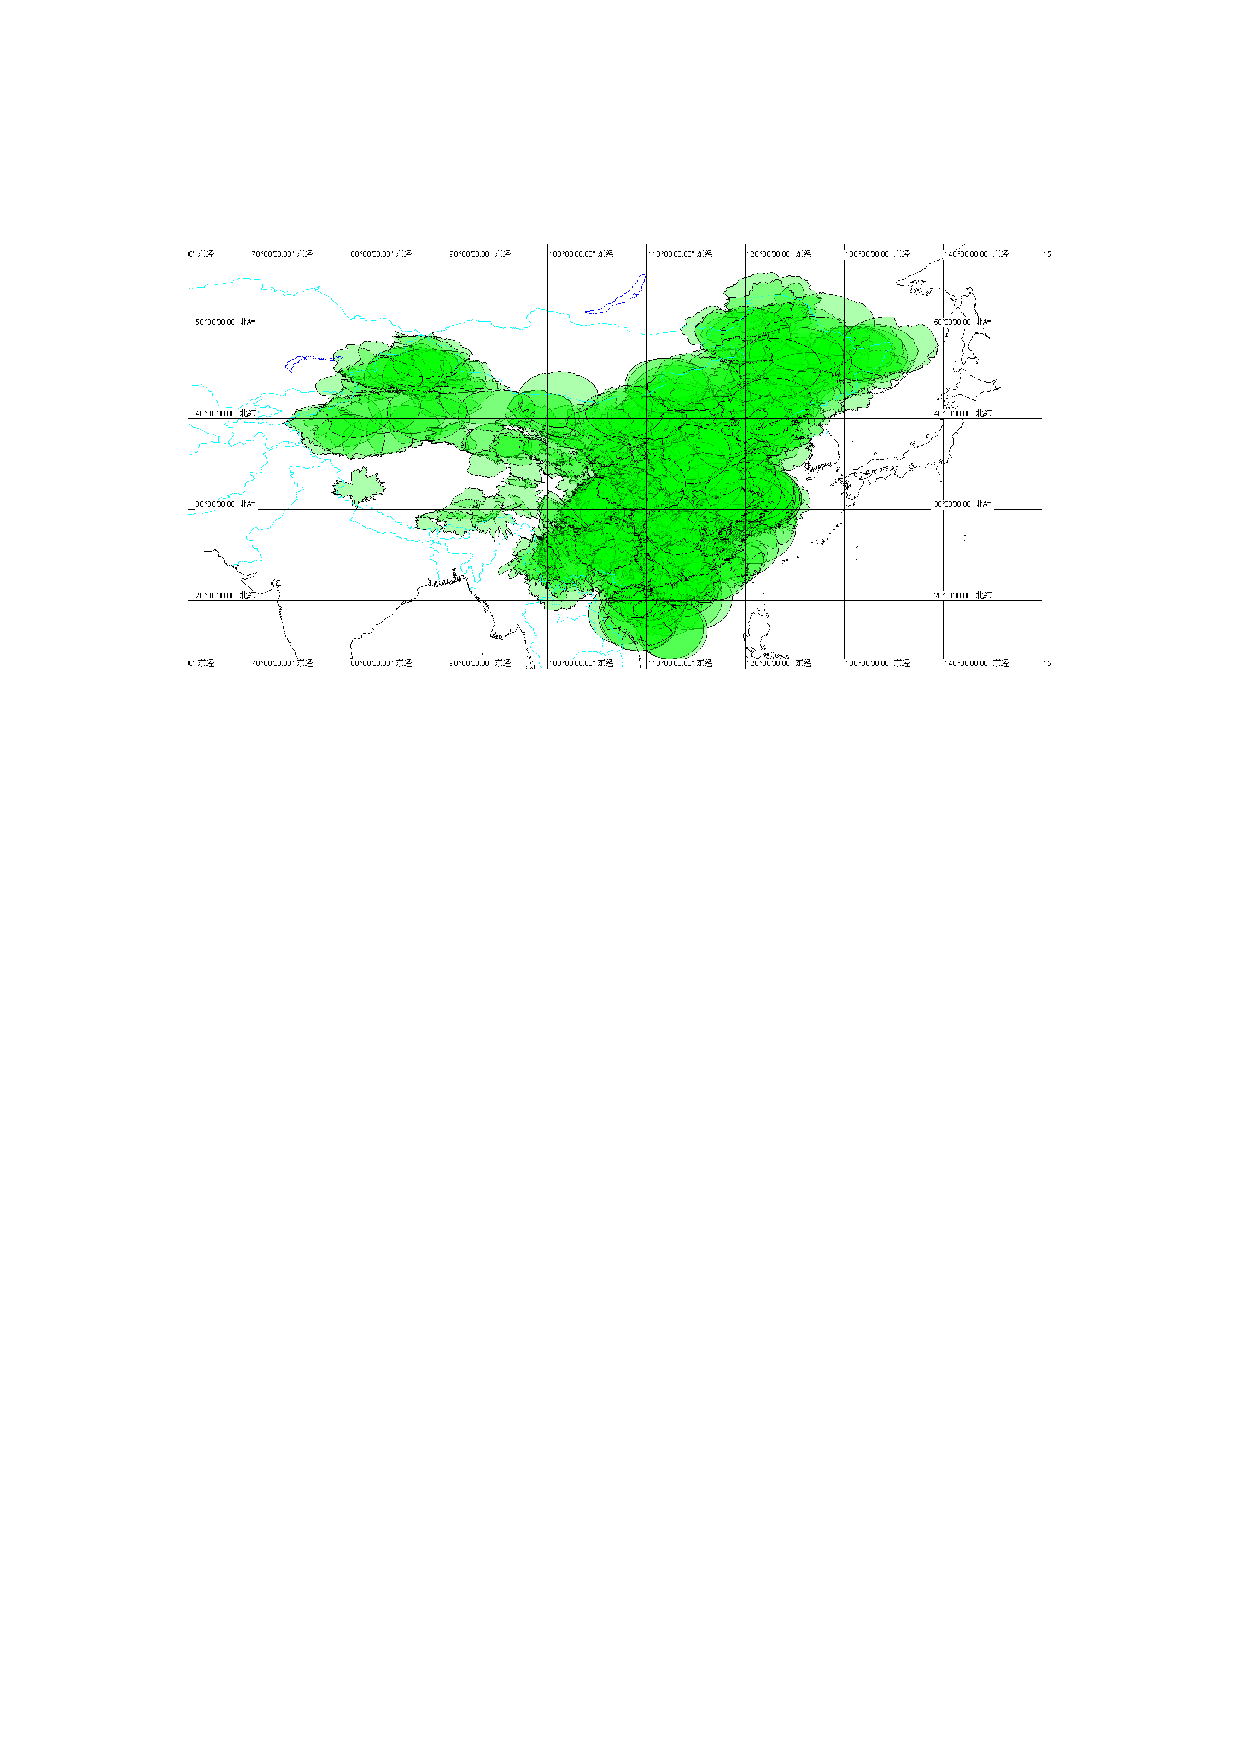
\includegraphics[width=12cm]{pic/china_8400m.pdf}
\caption{中国 8400m 空域 ADS-B 覆盖情况\protect\footnotemark}
\label{fig:china_8400m}
\end{figure}

\footnotetext{图片来源:参考文献\cite{e6}}

在中国南海,为满足 L642 路和 M771 路 ADS-B 监控控制需求,提升三亚 FIR 的 ADS-B 监控能力,CAAC 在 FIR 内增设了 4 个 ADS-B 站。截至 2016 年 4 月 19 日文档发布期间,已有 4 个 ADS-B 站和 1 个 ADS-B 数据处理站完成了安装调试和现场验收测试,空中交通管制自动化系统已完成软件升级测试,即将投入运作,这一地区的监测范围将大大改善。

中方愿将 ADS-B 数据处理中心的 ADS-B 数据与周边国家/行政部门共享。

根据 ICAO 东南亚第十四次会议和孟加拉湾区域 ADS-B 实施工作组会议信息论文(IP,Information Paper)显示\upcite{e7},自 2016 年起,中国一直在规划国家 ADS-B 项目,该项目由 308 个地面站和 3 级网络架构组成,用于处理和分发 ADS-B 数据。根据项目方案,所有的安装部署活动已经完成,所有的现场验收测试(SAT)和飞行检查将于 2018 年底完成。ADS-B 服务的初步运营将于 2019 年初准备就绪。2019 年 7 月 1 日,ADS-B 试运行全国空域。

\subsection{东南亚}

\subsubsection{印度尼西亚}



\subsubsection{马来西亚}

\begin{figure}[htbp]
\centering
\begin{minipage}[t]{0.48\textwidth}
\centering
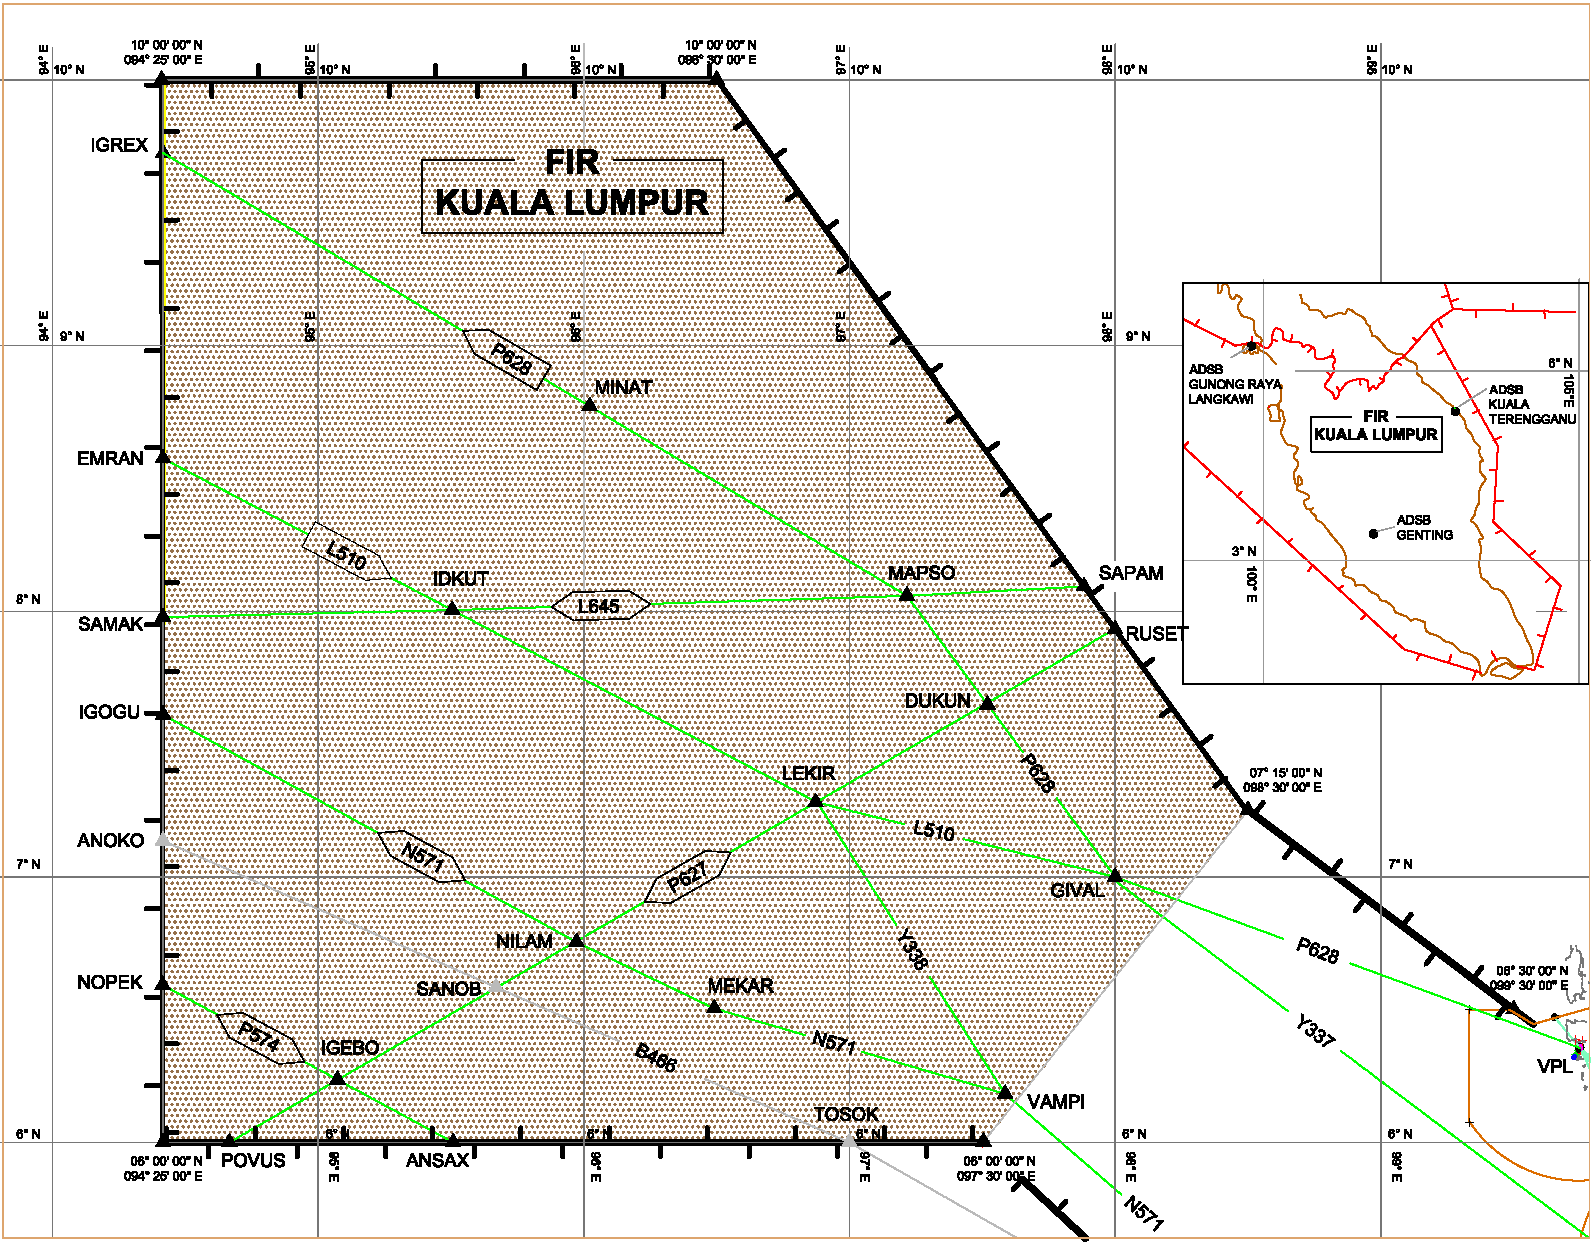
\includegraphics[width=8cm]{pic/malaysia_cover.png}
\caption{马来西亚}
\label{fig:malaysia_cover}
\end{minipage}
\begin{minipage}[t]{0.48\textwidth}
\centering
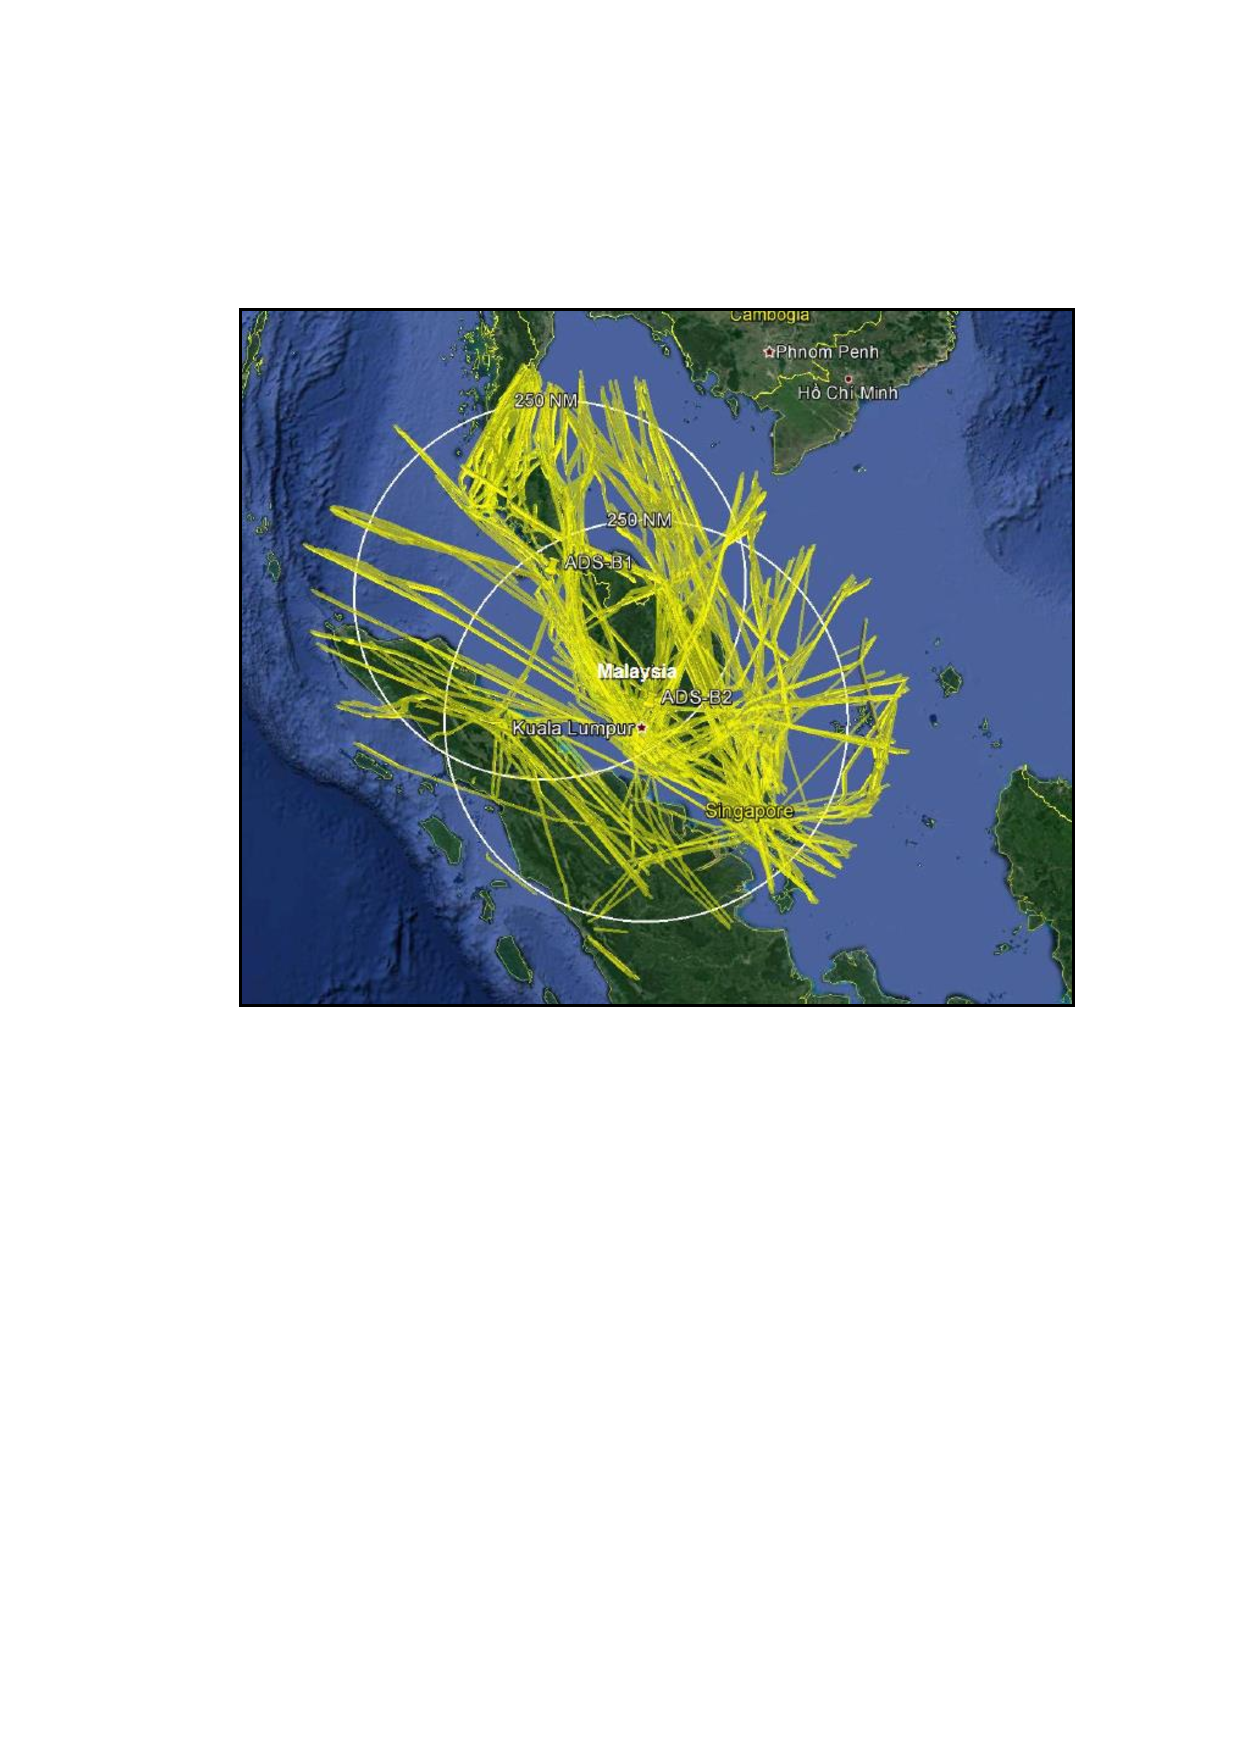
\includegraphics[width=7.5cm]{pic/Malaysia.pdf}
\caption{马来西亚航迹}
\label{fig:Malaysia}
\end{minipage}
\end{figure}

\begin{figure}[htbp]

\end{figure}

\subsubsection{泰国}

\begin{figure}[htbp]
\centering
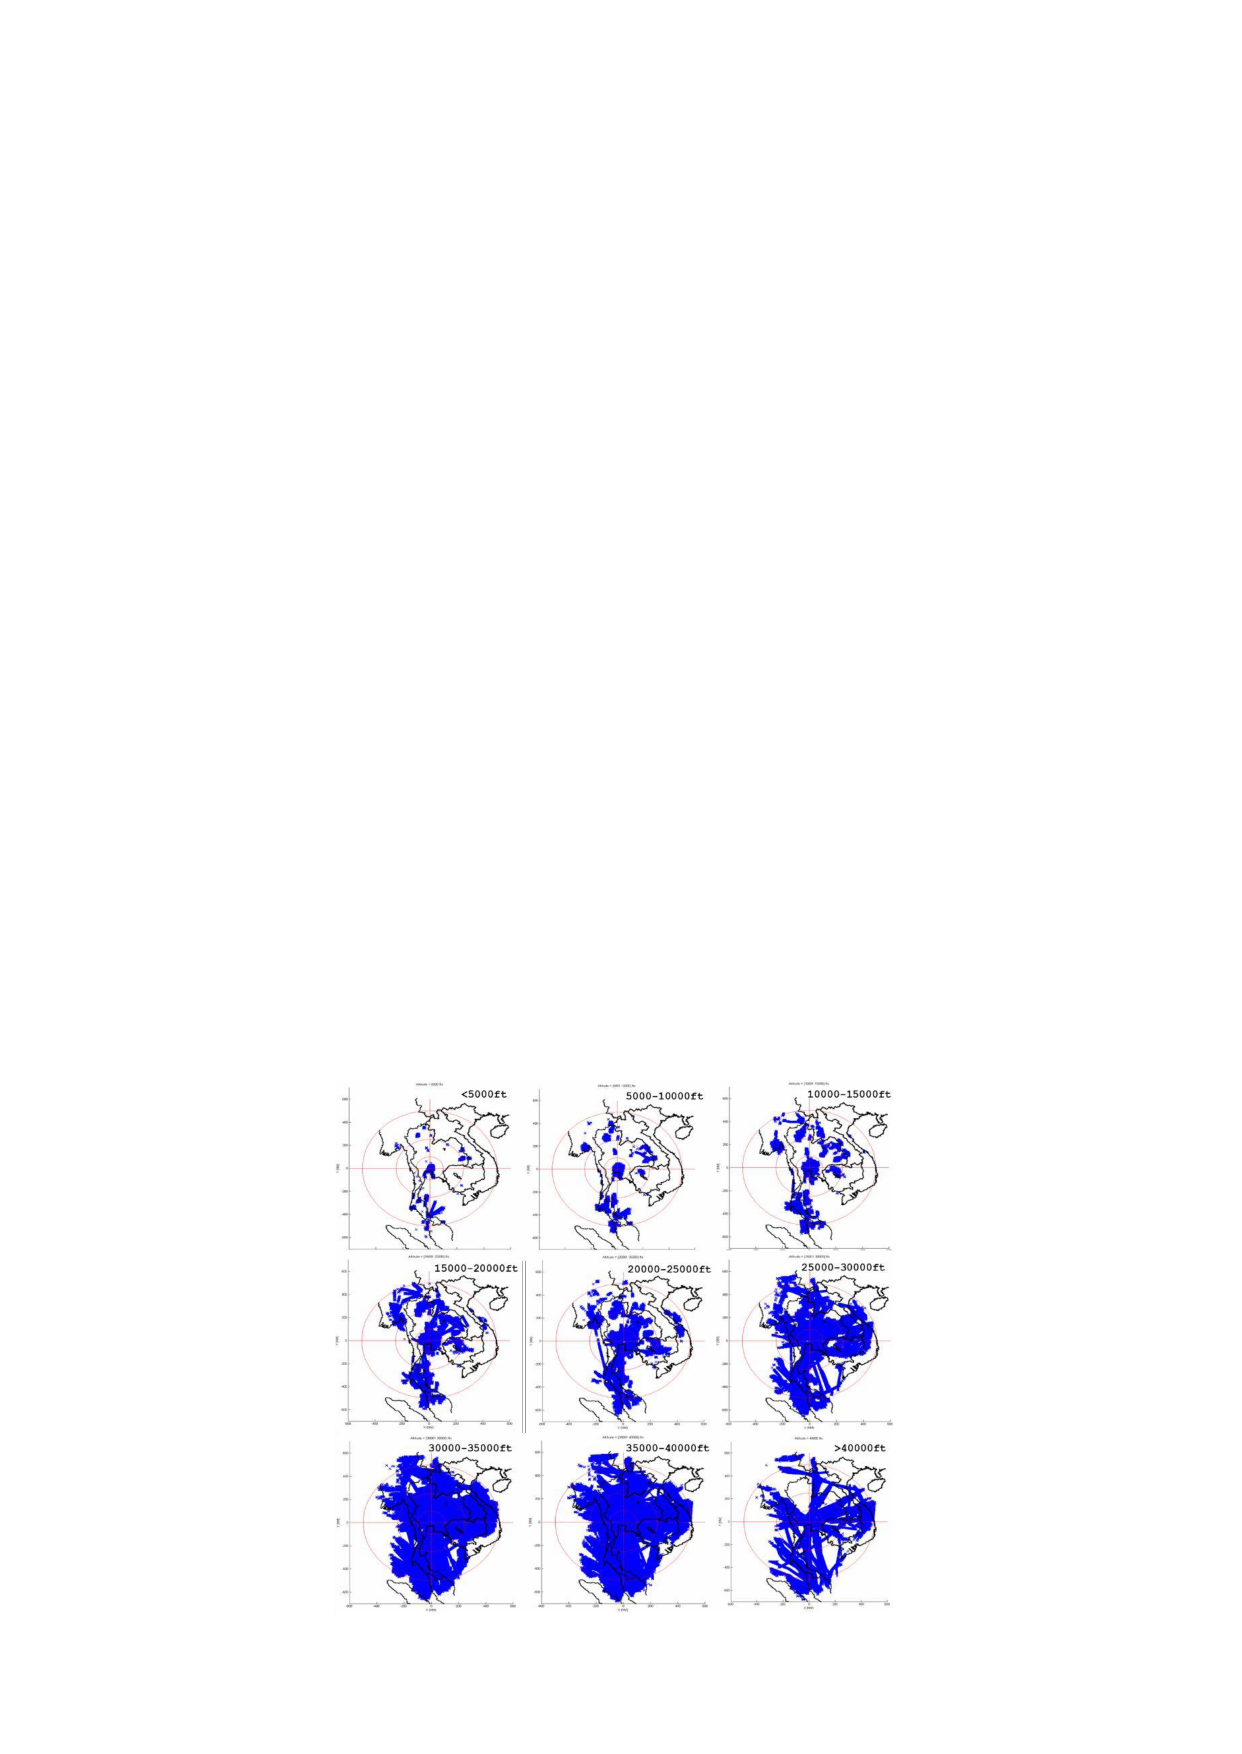
\includegraphics[width=13cm]{pic/thailand.pdf}
\caption{泰国}
\label{fig:thailand}
\end{figure}

\subsubsection{菲律宾}

\begin{figure}[htbp]
\centering
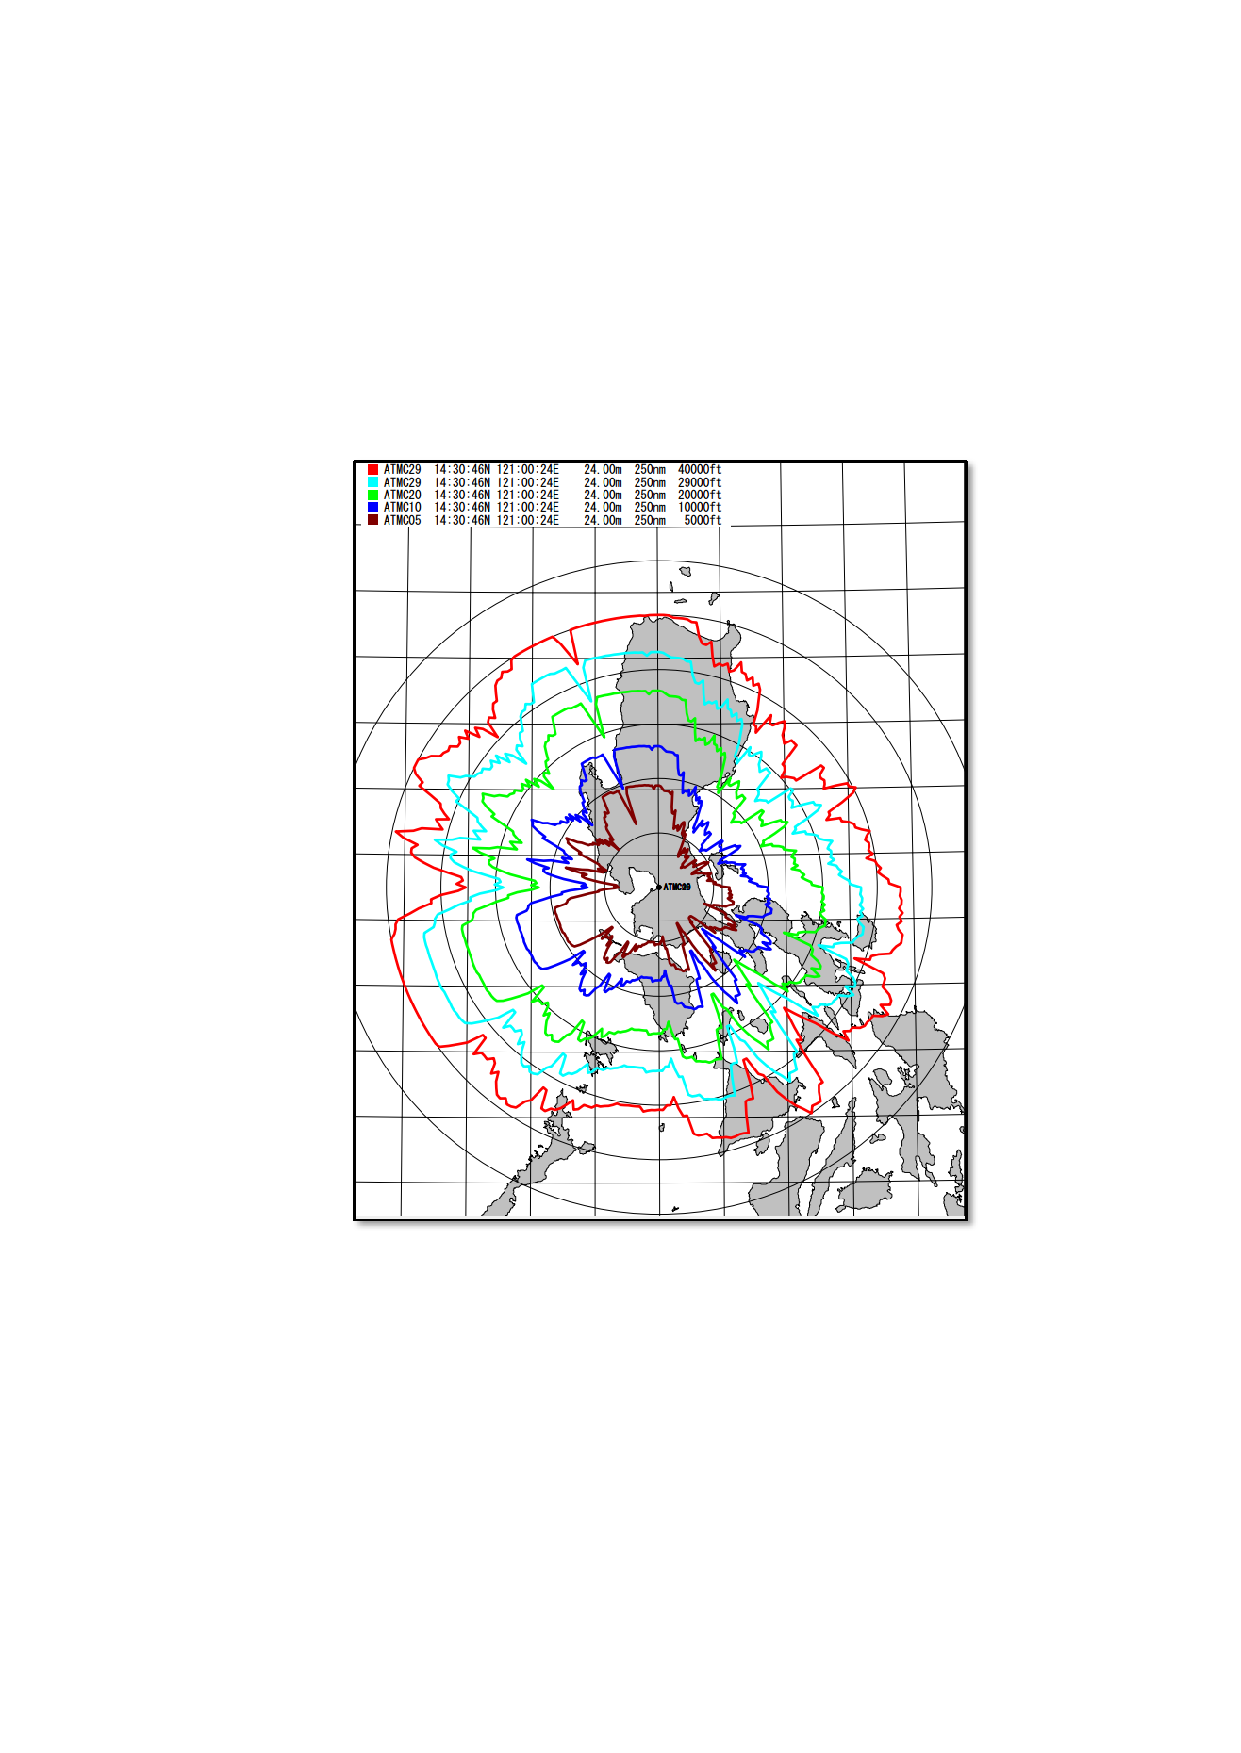
\includegraphics[width=7cm]{pic/phillipine.pdf}
\caption{菲律宾}
\label{fig:phillipine}
\end{figure}



